%Classe du document, A4, police taille 12
\documentclass[a4paper,12pt]{article}

% Dictionnaire français, pour caractères spéciaux, tirets, caractères accentués
\usepackage[french]{babel}
\usepackage[utf8]{inputenc}
%Toujours plus d'accents
\usepackage[T1]{fontenc}

\usepackage{indentfirst}
%Pour créer des paragraphes random
\usepackage{lipsum}
%bibliographie Le style dépend du projet, voir avec le grand chef A mettre à
%l'endroit où vous voulez la faire apparaitre Donc dans le code pas ici t'as vu
%\bibliographystyle{ieeetr} \bibligraphy{nom_du_fichier.bib}

%hauteur entre deux lignes
\baselineskip 200cm
%hauteur entre deux paragraphes
\parskip 2mm
%longueur d'indentation
\parindent 2mm
%(on utilise \indent et \noindent sinon)

%Gérer ses marges

%Facilement
\usepackage[margin=2cm]{geometry}

%Précisément \usepackage[left=2cm , right=2cm, bottom=2cm, top=2cm,
%headheight=2cm]{geometry} header c'est l'en-tête pas la marge supérieure

%Toujours plus précisément \addtolength{\oddsidemargin}{-0.5in}
%\addtolength{\evensidemargin}{-5cm} \addtolength{\topmargin}{-0.5in}

%Faires des articles  plusieures colonnes
\usepackage{multicol}
%Separation des colonnes
\setlength{\columnsep}{2cm}

%Commentaire sur plusieurs lignes
\usepackage{verbatim}

%Avoir des entêtes et pieds de page stylés
\usepackage{fancyhdr}
\pagestyle{fancy}
%Pour enlever l'entête avec les sections \fancyhf{}

%Ca se fait sous format \<pos><type>{<contenu>} type c'est "head" ou "foot" pos
%pour position gauche "l", droite "r" ou centre "c" contenu c'est ce que tu mets
%dans dedans marche aussi avec des images mais flemme mettre un trait
%\renewcommand{\footrulewidth}{1.5pt}

% Liens dans le document
\usepackage{hyperref}  
% Légendes dans les environnements "figure" et "float"
\usepackage{subcaption}
%La base pour faire des figures juste
\usepackage{graphicx}
\usepackage[export]{adjustbox}
\usepackage{wrapfig}
%Trucs utiles pour les maths
\usepackage{amsmath}

\begin{document}
\begin{titlepage}
    \begin{center}
        \vspace*{0.5cm}
        
\includegraphics[scale=0.1]{logo_ponts}\\
        \vspace{0.7cm}
        {\Large ÉCOLE NATIONALE DES PONTS ET CHAUSSÉES}\\
        \vspace{1cm}
        \rule\linewidth{0.05cm} {\huge Caractérisation du powercreep des jeux
        vidéo Pokémon \par} \rule\linewidth{0.05cm}
        \vspace{1cm}
        {\Large Statistiques numériques et analyse de données \par}
        \vspace{0.8cm}
        {\Large Par}\\
        \vspace{0.3cm}
        {\large \textit{DREVET Matthieu}}\\
        {\large \textit{ESTEVE Erwann}}\\
        {\large \textit{GOURGUE François}}\\
        {\large \textit{MALGAT Étienne}}\\
        {\large \textit{POLO Tidiane}}\\
        \vspace{1.2cm}
    \end{center}
\end{titlepage}
\tableofcontents
\newpage
\section{Introduction}
La série de jeux Pokémon, créée par Game Freak et éditée par Nintendo, a débuté
en 1996 avec les jeux Pokémon Rouge et Vert au Japon, avant de conquérir le
monde entier. L'univers Pokémon repose sur le concept de capture et
d'entraînement de créatures appelées pokémons, utilisées pour combattre d'autres
dresseurs. Le système de combat se joue au tour par tour, les pokémons
s'affrontant en un contre un, les joueurs pouvant ramener jusqu'à 6 pokémons.
Chaque jeu de la série se déroule dans une région différente du monde fictif de
Pokémon, présentant de nouveaux pokémons, des villes uniques et des défis
spécifiques. Aujourd'hui, Pokémon a été adapté pour de nombreux autres médias,
et la franchise Pokémon est aujourd'hui considérée comme la franchise la plus
lucrative de l'histoire.

La série principale de jeux Pokémon ne s'est pas arrêtée depuis 1996, et un
nouveau jeu est publié par Game Freak tous les 3 ans environ. Pour rendre chaque
nouveau jeu intéressant, il est créé de nouveaux pokémons, ayant un design
unique par rapport aux précédents (types, statistiques, capacités apprises...).
De plus, et afin d'inciter les joueurs à acheter le jeu, l'éditeur a tendance à
augmenter la "puissance" des nouveaux pokémons afin de leur donner un interêt
par rapport aux anciens : l'augmentation de la "puissance" des pokémons (en
moyenne) est nommé powercreep. Ce phénomène est dénoncé par certains joueurs,
qui voient leurs pokémons favoris devenir plus obcelète de génération en
génération. 

Ce phénomène de powercreep est au coeur de notre projet. Nous allons chercher à
déterminer quels changements ont eu lieu dans le design des nouveaux pokémons au
fil des générations, et dans quel mesure ces changements peuvent expliquer le
phénomène de powercreep.

\begin{figure}[!h]
    \centering
    
\includegraphics[width=0.6\textwidth]{Image/scarlet-violet.jpg}
    \caption{\textit{Pokémon Écarlate et Violet}, 2 derniers opus de la série,
    incluant 120 nouveaux pokémons et de nombreux anciens. Ces jeux constituent
    la $9^{e}$ génération de la saga ($9^{e}$  jeux ajoutant de nouveaux
    pokémons.)}
    \label{fig:image1}
\end{figure}

La première base de donnée décrit les différentes statistiques des pokémons
(base stats, qui sont des bytes, types qui sont des catégories, génération
d'appartenance...), la seconde sont les statistiques d'usages des pokémons sur
le simulateur de combat \textit{Pokemon Showdown!}, qui est utilisé par les
joueurs-compétiteurs des jeux Pokémon. Ces deux jeux de données nous permettent
de vérifier ce qui, dans le design d'un pokémon, donne sa viabilité (autrement
dit sa puissance). 

\newpage
\section{Description des mécaniques de jeu et des données}
\subsection{Explication sur le déroulement d'une partie et l'influence des données}

Avant de chercher les origines du phénomène de powercreep, il nous faut évaluer
quelles données influent sur la viabilité d'un pokémon. 4 données sont en
général retenues pour décrire un pokémon :

\begin{itemize}
    \item Ses \textbf{statistiques}, qui sont encodées sur un octet et sont
    divisées entre HP (\textit{Health Points}, "points de vie" en français),
    Attaque, Défense, Attaque Spéciale, Défense Spéciale et Vitesse. Ces données
    quantitatives influent sur la puissance offensive et défensive des Pokémon.
    \item Son \textbf{double-type} (un pokémon peut avoir 1 ou 2 types parmi
    18), qui vont interagir avec les attaques reçues et subies (chaque attaque
    est associée à un type, qui intéragira avec celui du lanceur et de la cible)
    \item L'ensemble des capacités qu'il peut apprendre, appelé
    \textbf{movepool}. Les capacités (parfois nommées "attaques" lorsqu'elles
    infligent des dégâts au pokémon adverse) sont les actions réalisables par
    les pokémons une fois sur le terrain. Certaines capacités sont uniques,
    d'autres sont accessibles par plusieurs pokémons.
    \item Ses \textbf{talents}, qui sont des pouvoirs particuliers qui se
    manifestent en combat. Certains talents sont uniques, d'autres sont
    accessibles par plusieurs pokémons. Une espèce de pokémon peut en avoir
    jusqu'à 3 différents, mais chaque individu n'en a qu'un seul.
\end{itemize}

\begin{figure}[!h]
    \centering
    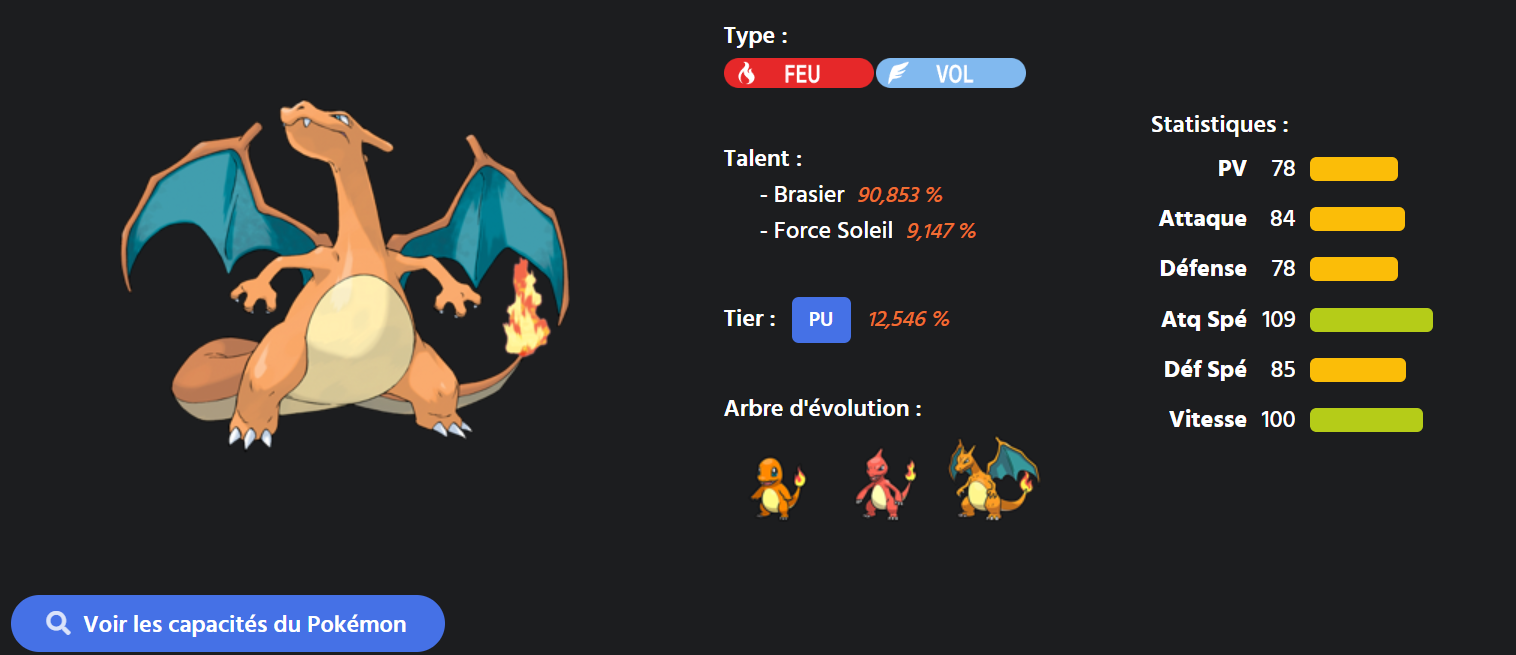
\includegraphics[width=0.6\textwidth]{Image/dracaufeu_coup_critique.png}
    \caption{Page du site coupcritique.fr (site d'analyse stratégique Pokémon)
    dédiée à Dracaufeu. On y retrouve immédiatement les données citées
    précédemment.}
    \label{fig:image2}
\end{figure}

Une explication rapide du déroulement d'une partie s'impose (certains points,
non essentiels à la compréhension, seront passés):
\begin{enumerate}
    \item Avant le début du combat, chaque joueur \textbf{choisit} son équipe
    d'au plus \textbf{6 pokémons} (en général 6, puisqu'il n'y a aucun intéret à
    en jouer moins). Il choisit pour chaque pokémon \textbf{4 capacités} parmis
    celles que le pokémon peut apprendre et un de ses talents (s'il en a
    plusieurs disponibles, il faut en choisir un).
    \item Au début du combat, chaque joueur sélectionne le \textbf{premier
    pokémon} à être envoyé sur le terrain.
    \item L'objectif du match est d'\textbf{amener les points de vie} (noté PV
    ou HP pour \textit{Health Points}) de chacun des pokémons de l'adversaire
    \textbf{à 0}. Chaque tour, chaque joueur doit choisir d'executer une des 4
    capacités de son pokémon actif (qui pourra par exemple retirer des points de
    vie au pokémon adverse actif), ou de changer de pokémon actif pour un autre
    de ses 6 pokémons (ce qu'on appelle \textit{switch}). Le joueur agissant en
    premier est déterminé à la fois par la statistique de vitesse des pokémons
    actifs et un système de "priorité" (qu'on ne détaillera pas, celui-ci se
    limitant en général au fait qu'un changement de pokémon se fait avant
    n'importe quelle capacité de l'adversaire). Les capacités peuvent avoir
    divers effets, mais 3 catégories sont importantes à retenir :
          \begin{itemize}
              \item les capacités \textbf{physiques}, qui font baisser les
              points de vie du pokémon adverse actif en fonction de la
              "puissance" de la capacité (appelée \textit{base power}, propre à
              la capacité), des types de la capacité, du lanceur et de
              l'adversaire, et des statistiques respectivement d'attaque du
              lanceur et de défense de l'adversaire
              \item les capacités \textbf{spéciales}, semblablent aux capacités
              physiques mais qui se basent sur les statistiques d'attaque
              spéciale du lanceur et de défense spéciale de l'adversaire.
              \item les capacités de \textbf{statut}, qui provoquent d'autres
              effets et ne se basent sur aucune statistique en particulier.
          \end{itemize}
\end{enumerate}

\begin{figure}[!h]
    \centering
    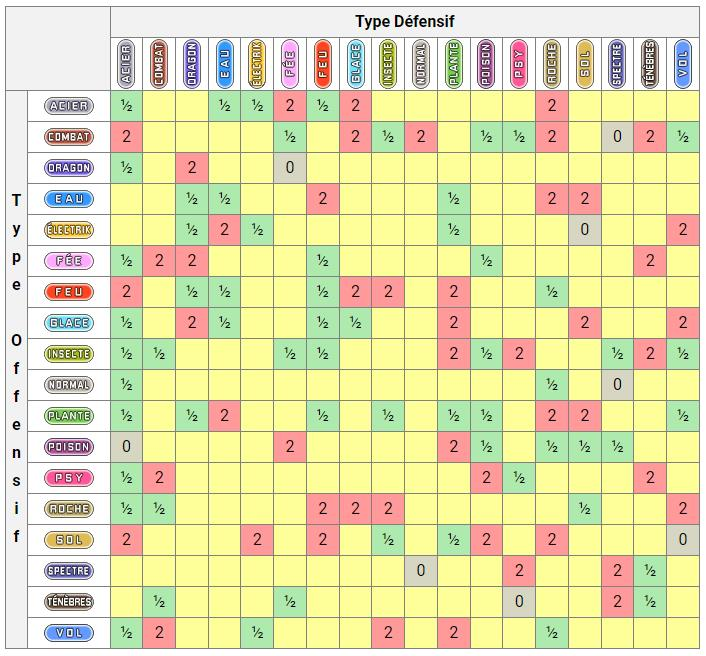
\includegraphics[width=0.6\textwidth]{Image/table-des-types-pour-pokemon-arceus.jpg}
    \caption{Table des types, donnant les modificateurs sur les dégâts infligés
    par une capacité physique ou spéciale en fonction du type de l'attaque et de
    l'adversaire. Ainsi, une capacité de type Feu infligera 2x plus de dégâts
    sur un pokémon de type Plante, tandis qu'elle infligera 2x moins de dégats
    sur un pokémon de type Eau.}.
    \label{fig:tabletype}
\end{figure}

Les dégâts infligés par les attaques physiques ou spéciales sont calculés via la
formule suivante (version simplifiée) :
\begin{equation}
    PV_{perdus}=\lfloor ( \lfloor \frac{\lfloor \frac{\lfloor 100*0.4+2 \rfloor * Atk * BasePower}{Def}\rfloor}{50}\rfloor +2)*CM \rfloor
\end{equation}
Avec :
\begin{itemize}
    \item $Atk$ la statistique offensive du lanceur (respectivement l'attaque
    pour une capacité physique, l'attaque spéciale pour une capacité spéciale)
    \item $Def$ la statistique défensive du pokémon adverse (respectivement la
    défense pour une capacité physique, la défense spéciale pour une capacité
    spéciale)
    \item $BasePower$ la puissance de la capacité
    \item $CM$ un coefficient comprenant les modificateurs liés aux interactions
    de type (voir la table~\ref{fig:tabletype}), le \textit{STAB} (modificateur
    augmentant la puissance d'une capacité ayant le même type que son lanceur),
    un potentiel Coup Critique (augmentation aléatoire des dégats)...
\end{itemize}

Ce qu'il faut retenir :
\begin{itemize}
    \item Les statistiques d'\textbf{attaque} et d'\textbf{attaque spéciale}
    (qu'on notera Atk et Sp.Atk) influent positivement sur les dégats infligés
    par les capacités \textbf{physiques} ou \textbf{spéciales} lancées par le
    pokémon
    \item Les statistiques de \textbf{défense} et de \textbf{défense spéciale}
    (qu'on notera Def et Sp.Def) réduisent les dégats reçus lorsque le pokémon
    subit une capacité \textbf{physique} ou \textbf{spéciale}.
    \item La statistique \textbf{HP} donne le \textbf{nombre de point de vie}
    d'un pokémon au début du combat (qui représente sa capacité à encaisser des
    capacités sans tomber KO).
    \item La statistique de \textbf{vitesse} (qu'on notera Spe ou Speed) donne
    l'\textbf{ordre des actions} au sein d'un tour (quel pokémon va executer sa
    capacité en premier).
\end{itemize}

Notons que certaines données influant rarement sur les combats, comme le sexe
des pokémons ou leur poids, ne seront pas pris en compte, car leur influence sur
la viabilité d'un pokémon est négligeable.

\subsection{Présentation du jeu de données}
Le tableau \textit{Pokemon.csv} contient, pour chaque pokémon, ses statistiques,
ses types, sa génération d'origine et un attribut "Can\_Evolve", qui indique si
le pokémon peut encore évoluer ou non (les pokémons utilisés en compétitions
sont, sauf exceptions, entièrement évolués). Il contient donc une partie des
données étudiées définissant la viabilité d'un pokémon.

Le second jeu de donnée provient du document \textit{gen9ou-0.json} (fourni par
le simulateur \textit{Pokémon Showdown!}). Une rapide explication du format
compétitif joué sur le site est nécessaire afin de comprendre ce document.

Le format compétitif principal, nommé \textit{OU} pour \textit{OverUsed}, est un
format reprenant les combats entre joueurs disponibles dans les jeux pokémons.
La plupart des pokémons sont autorisés, les pokémons bannis sont en général les
pokémons dit \textit{légendaires} (qui font figure d'objectif final de
l'aventure des jeux, et ont des statistiques largement supérieures aux autres
pokémons), et d'autres pokémons bannis via des votes de la communauté de
joueurs. Certaines règles s'appliquent en plus (interdiction de jouer deux fois
le même pokémon, interdiction d'infliger le statut "sommeil" à plus de 1 pokémon
adverse...), et le combat se déroule selon l'explication plus haut. Les joueurs
sont classés via un système d'ELO similaire à celui utilisé pour les échecs.

Le simulateur garde certaines données de chaque partie jouée sur le site et,
chaque mois, fourni ces données collectées sur le mois précédent. Ces données,
contenues dans le document \textit{gen9ou-0}, contiennent notament :
\begin{itemize}
    \item le nombre total de combat joué
    \item le nombre d'occurences de chaque pokémon
    \item le nombre d'occurences de chaque capacité par pokémon
    \item le nombre d'occurences de chaque talent par pokémon
\end{itemize}
Ces données complètent alors des données manquantes de \textit{Pokemon.csv}. On
fera les deux approximations suivantes :
\begin{itemize}
    \item le taux d'utilisation d'un pokémon représente sa viabilité ou
    "puissance"
    \item les seules capacités influant sur la viabilité d'un pokémon sont
    celles ayant déjà été utilisées sur le simulateur (étant donné que le nombre
    de parties jouées est de l'ordre du million, on peut considérer que toutes
    les capacités "utiles" des pokémons ont été utilisées au moins une fois)
\end{itemize}
\section{Description et analyse des données}
\subsection{Description des données}
Avant de chercher à caractériser le powercreep, il est nécessaire de pouvoir
prouver son existence. Pour cela, nous pouvons nous intéresser à l'évolution de
l'usage des pokémons par génération. En effet, si le powercreep existe, on
devrait observer une augmentation de l'usage des pokémons des générations les
plus récentes. L'image ci-dessous représente l'évolution de l'usage moyen des
pokémons par génération, en utilisant les données de \textit{gen9ou-0.json} :
\begin{figure}[!h]
    \centering
    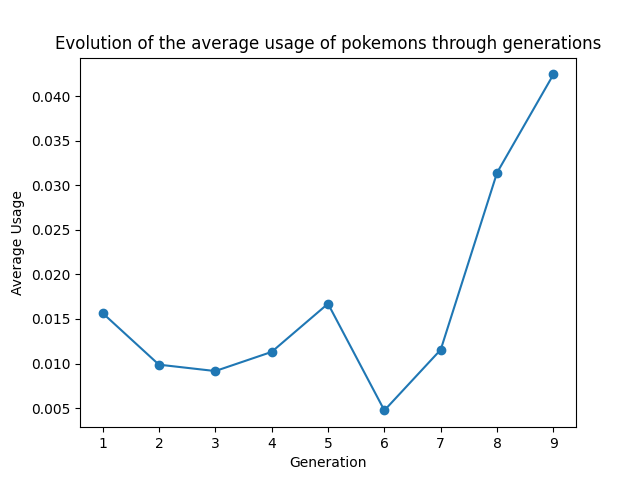
\includegraphics[width=0.6\textwidth]{Image/avg_usage_by_generation.png}
    \caption{Évolution de l'usage moyen des pokémons par génération}
    \label{fig:image4}
\end{figure}

On constate que, s'il n'y a pas de net corrélation entre taux d'usage et
génération lors des 7 premières générations, les générations 8 et 9 ont un taux
d'usage moyen supérieur aux générations précédentes. On peut donc affirmer que
le powercreep existe bien sur les dernières générations.\\
N.B. : La baisse d'usage des pokémons de génération 6 et 7 par rapport aux
générations précédentes s'explique par le fait que certains pokémons n'était pas
encore disponible sur le simulateur/dans les jeux lorsque les données ont été
collectées. En particulier, la génération 7 possède de nombreux pokémons qui
auraient été joués, mais qui sont restés exclusif à leur jeu d'origine.


Maintenant que nous avons vu que le phénomène de powercreep s'appliquait bien
aux jeux pokémons, nous pouvons nous intéresser à comment le design des pokémons
a évolué pour provoquer ce powercreep.

La façon la plus simple qu'aurait Game Freak (développeur des jeux Pokémon) pour
augmenter la puissance des pokémons des nouvelles générations par rapport aux
anciens serait d'augmenter le total de statistiques des nouveaux pokémons. En
effet, les statistiques des pokémons sont les seuls données strictement
"positive" pour un pokémon :  un type donnent les résistances mais aussi les
faiblesses d'un pokémon, tandis que les talents sont très différents les uns des
autres et donc parfois difficilement comparables (un talent améliore souvent
certains aspects par rapport à d'autres).

On peut donc s'intéresser à l'évolution de la moyenne du total de statistiques
des pokémons par génération :

\begin{figure}[htbp]
    \centering
    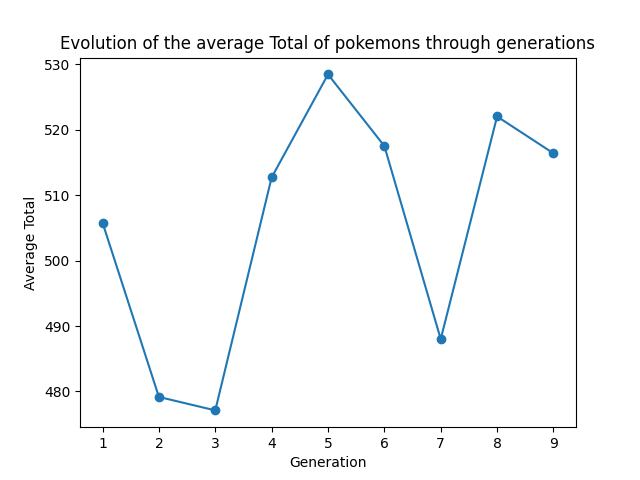
\includegraphics[width=0.6\textwidth]{Image/avg_total_per_generation.png}
    \caption{Évolution du total de statistique moyen en fonction de la
    génération}.
    \label{fig:image5}
\end{figure}
\newpage
On constate que le total de statistique moyen ne semble pas être la raison de
l'augmentation d'usage des pokémons de dernière génération : les moyennes des
générations 8 et 9 (qui, nous l'avons vu précédemment, ont introduit les
pokémons les plus viables) sont semblables à celle des génération 4-5-6, dont
les usages sont nettement plus bas.

Une autre tendance intéressante à vérifier concernant les statistiques des
pokémons est l'évolution de la variance inter-statistique. En général, un
pokémon ayant des statistiques très déséquilibrées (par exemple, un pokémon
ayant des statistiques d'attaque et de vitesse très élevées et toutes les autres
très faibles) sera plus viable qu'un pokémon ayant des statistiques plus
lissées, car le premier pourra plus facilement se justifier un rôle au sein
d'une équipe. On peut donc s'intéresser à l'évolution de la moyenne sur les
génération de la variance entre les 6 statistiques :

\begin{figure}[htbp]
    \centering
    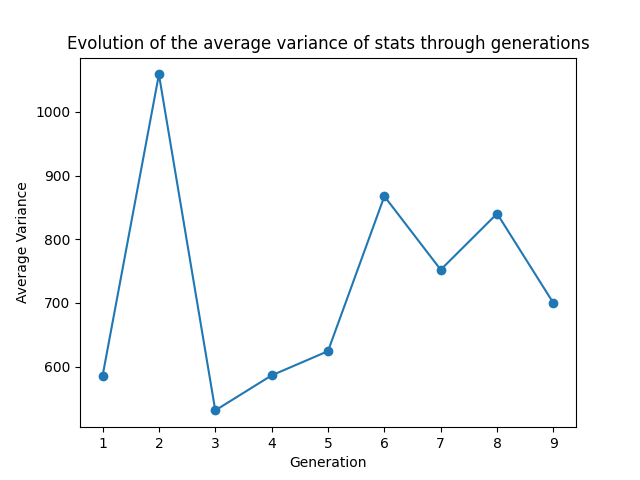
\includegraphics[width=0.6\textwidth]{Image/avg_var_stats_per_generation.png}
    \caption{Évolution de la variance moyenne des statistiques en fonction de la
    génération}.
    \label{fig:image6}
\end{figure}

Une fois de plus, on ne peut expliquer le powercreep des dernières générations
par cette donnée : en effet, les statistiques des pokémons originaires de la
deuxième génération sont fortement déséquilibrées et pourtant, leurs usages sont
parmis les plus bas. Il faut donc chercher la cause du powercreep sur d'autres
aspects du design des pokémons.

\subsection{Réduction de la dimentionnalité}
Comme nous l'avons vu précédemment, les données associées sont à la fois des
données quantitatives (statistiques) et qualitatives (types, capacités,
talents). Nous avons choisi de réduire la dimentionnalité des données à l'aide
des méthodes d'analyse en composantes principales et d'analyse des
correspondances multiples.

\subsubsection{Réduction de la dimentionnalité sur les statistiques}
Les statistiques d'un pokémon sont des données quantitatives, nous pouvons donc
appliquer une Analyse en Composantes Principales classique. Notons que notre
espace d'origine comprend 6 dimensions pour les 6 statistiques d'un pokémon (HP,
Attaque, Défense, Attaque Spéciale, Défense Spéciale et Vitesse). Les figures
ci-dessous contiennent des informations obtenues à partir de l'ACP :

\begin{figure}[htbp]
    \centering
    \begin{minipage}[b]{0.45\textwidth}
        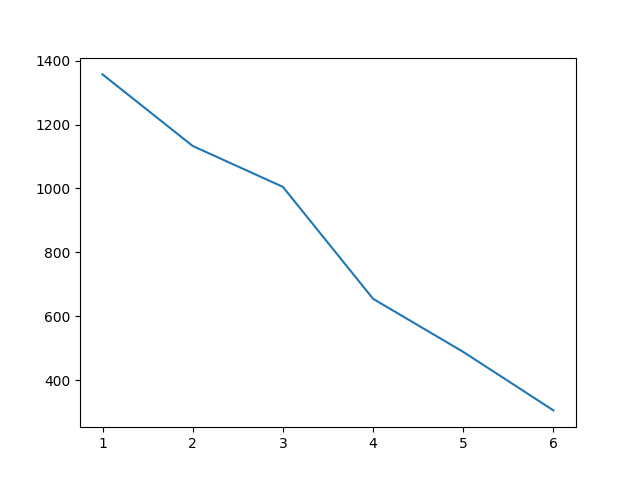
\includegraphics[width=\textwidth]{Image/explained_variation_PCA.png}
        \caption{Valeurs propres associées aux vecteurs propres de l'ACP}
    \end{minipage}
    \hfill
    \begin{minipage}[b]{0.45\textwidth}
        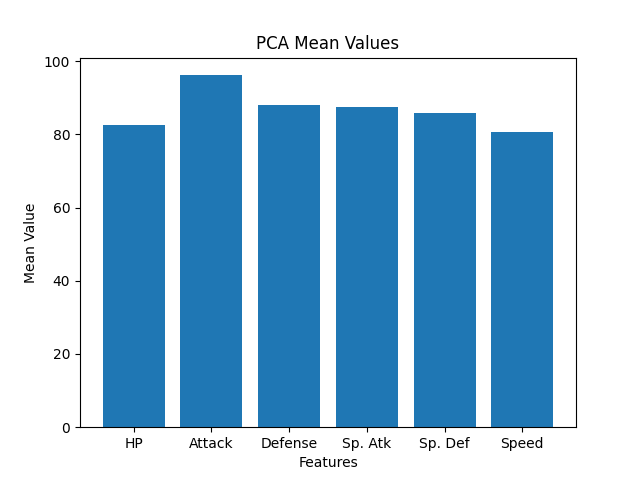
\includegraphics[width=\textwidth]{Image/mean_vector_PCA.png}
        \caption{Vecteur moyen (moyenne de chaque statistique)}
    \end{minipage}
    
    \vspace{0.5cm}
    
    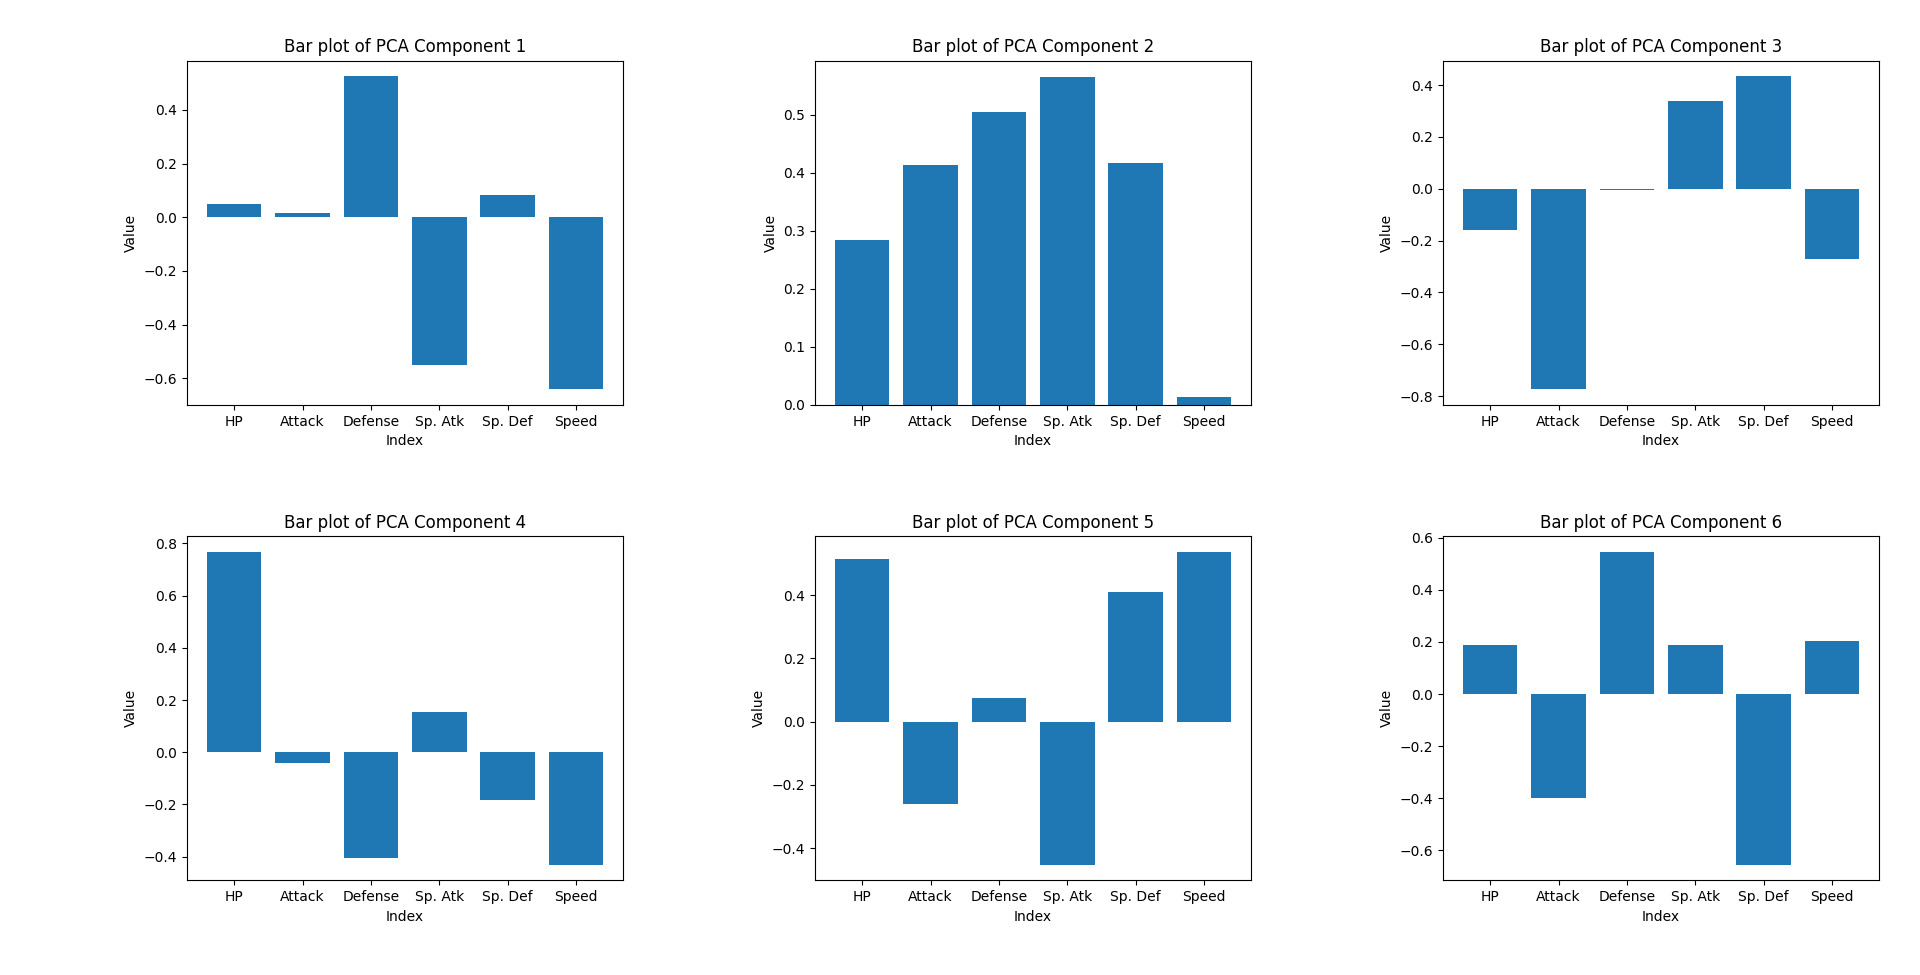
\includegraphics[width=0.8\textwidth]{Image/eigen_vector_PCA.png}
    \caption{Vecteur propre de l'ACP}
\end{figure}

On constate qu'il n'est pas vraiment pertinent de réduire la dimentionnalité des
statistiques : en effet, la Figure 4 ne permet pas de distinguer un "angle" sur
la courbe des valeurs prores, qui se situe en général à la dimension à partir
desquels la perte d'information par dimension réduite est importante. Cela
s'explique facilement par le fait que les 6 statistiques sont fortement
indépendantes entre les pokémons : s'il peut exister certains "patterns" dans
les répartitions de statistiques (voir la partie concernant le Clustering), il
n'y a pas de correlations systématiques entre les catégories de statistique. \\
On peut tout de même remarquer au sein des vecteurs propres (Figure 6) des
habitudes de design :
\begin{itemize}
    \item Les vecteurs 1 et 3 montrent une tendance qu'ont les pokémons ayant
    une forte défense à avoir une faible attaque spéciale et vitesse, tandis que
    les pokémons ayant une statistique importante d'attaque tendent à avoir des
    statistiques spéciales (Sp. Atk, Sp. Def) faibles.
    \item Le vecteur 2 montre des composantes positives dans toutes les
    statistiques sauf en vitesse (qui est quasi nulle) : la composante selon ce
    vecteur des pokémons dit "légendaires", qui ont de très hautes statistique
    en général, sauf leur vitesse qui est souvent moyenne, doit être grande et
    le nombre important de sorte de pokémons légendaires aux statistiques
    similaires justifie la forme de ce vecteur.
\end{itemize}
\subsubsection{Réduction de la dimentionnalité sur les types et les capacités}
Tous les pokémons ne peuvent pas apprendre les mêmes capacités dans les jeux
vidéos Pokémon. L'objectif de cette partie est d'étudier quelles capacités les
pokémons d'un type de pokémon peuvent apprendre. L'intérêt de cette partie est
double:   
\begin{itemize}
    \item 
    Tout d'abord, il s'agit de confirmer l'intuition que les pokémons d'un type
    peuvent apprendre des capacités associées au même type. 
    \item Ensuite, nous souhaitons visualiser le principe de \textit{coverage}
    (ou \textit{couverture d'option}): à priori, si un pokémon de type Feu doit
    en affronter un autre, il ne peut pas utiliser de capacités de type Feu pour
    vaincre de manière efficace son adversaire car les capacités de type Feu
    sont résistées par les pokémons ayant le type Feu (voir la
    table~\ref{fig:tabletype}). Il vaut mieux qu'il possède des capacités
    efficaces pour attaquer un pokémon de type Feu: les capacités du type Eau
    sont un bon exemple, on dira alors que le type Eau est un bon
    \textit{coverage} au type Feu. Cependant, selon le type de pokémon étudié,
    il est possible que des choix de design implique qu'un type possède une
    mauvaise coverage. 
\end{itemize}
Deux jeux de données binaires sont utiles ici: un premier qui contient les
pokémons en entrée et les types des pokémons en colonne, un second qui contient
les pokémons en entrée et les capacités qui sont pourraient ou non être apprises
par ces pokémons en colonne. Le premier jeu de données sert à classifier les
pokémons selon leur type afin de raisonner type par type dans l'analyse du
second jeu de données.

Le second jeu de données contient 592 colonnes (toutes les capacités des jeux
vidéos Pokémon). Cette dimension étant importante, nous avons choisi de la
réduire grâce à l'analyse des correspondances multiples (ACM). Nous avons choisi
cette méthode puisque les données étaient binaires donc assimilables à des
données qualitatives dont les seules modalités sont 0 et 1. 

Afin de choisir la nouvelle dimension, nous utilisons le diagramme d'éboulis des
valeurs propres. Etant donné que le jeu de données utilisé contient 291 entrées
(pokémons) et 592 colonnes, la dimension maximale du nouvel espace ne peut
dépasser 291. 
\newpage
\begin{figure}[!h]
    \centering
    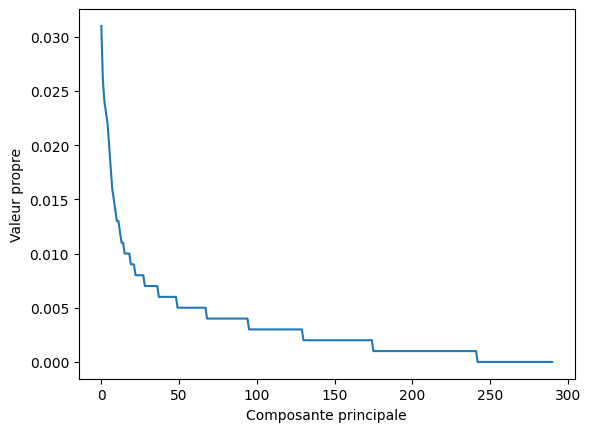
\includegraphics[width=0.5\textwidth]{eboulis_MCA.png}
    \caption{Diagramme d'éboulis des valeurs propres}.
\end{figure}

On remarque que la rupture de pente de la courbe se trouve vers la 25$^{e}$
composante. C'est donc la dimension qu'on choisit.

L'objectif est maintenant de trouver si certains axes propres représentent bien
certains types de pokémons. Pour cela, on regarde comment s'expriment les
pokémons en fonction des composantes. Si les pokémons d'un même type ont tous
une composante forte selon un axe propre et que les pokémons des autres types
ont tous une composante faible selon ce même axe, alors la composante représente
bien les pokémons du type trouvé. 

Jusqu'à la fin de la section, nous allons prendre l'exemple de la 3$^{e}$
composante qui contient des résultats satisfaisants et intuitifs. Pour cette
composante, on obtient la boîte à moustache suivante: 
\begin{figure}[!h]
    \centering
    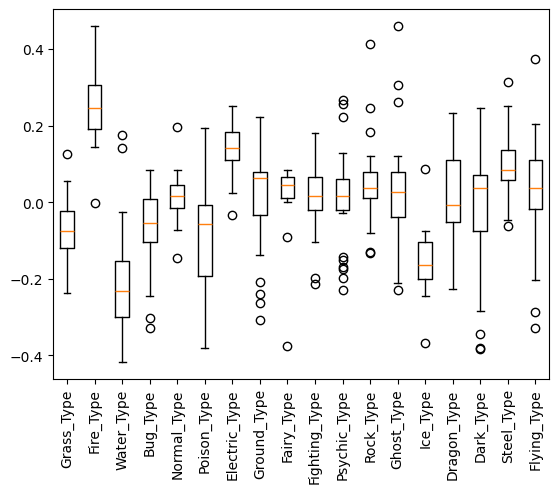
\includegraphics[width=0.5\textwidth]{moustache_MCA.png}
    \caption{Représentativité du 3e axe dans la construction des pokémons,
    classés par type}.
\end{figure}

On remarque que les pokémons de type Feu ont une forte composante selon le
3$^{e}$ axe. Par ailleurs, on voit que les pokémons de type Eau sont peu
représentés sur cet axe. Ce résultat est cohérent avec le design du jeu qui veut
que les pokémons de type Feau et Eau soient opposés. 

Maintenant que l'on sait que le 3$^{e}$ axe représente surtout les pokémons de
type Feu, on peut voir quelles capacités ont permis de construire ce 3$^{e}$
axe. Cela nous permet de trouver quelles capacités sont utilisées par les
pokémons de type Feu. Le résultat découle de la matrice des contributions. On
peut par exemple afficher les 30 capacités qui ont le plus contribué à
construire le 3$^{e}$ axe et les 30 capacités qui y on le moins contribué:
\begin{figure}[!h]
    \centering
    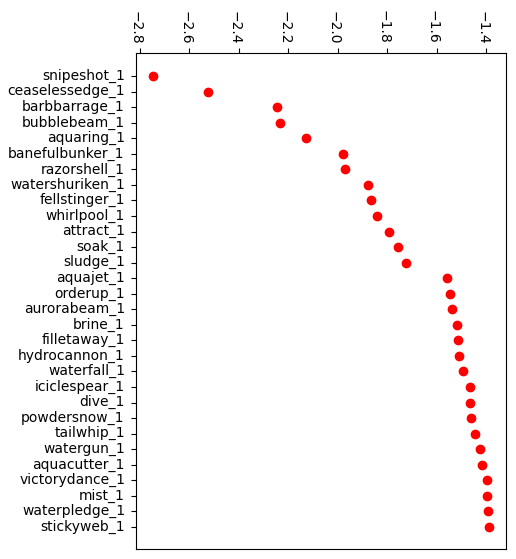
\includegraphics[width=0.4\textwidth]{bottom_attaques_MCA.png}
    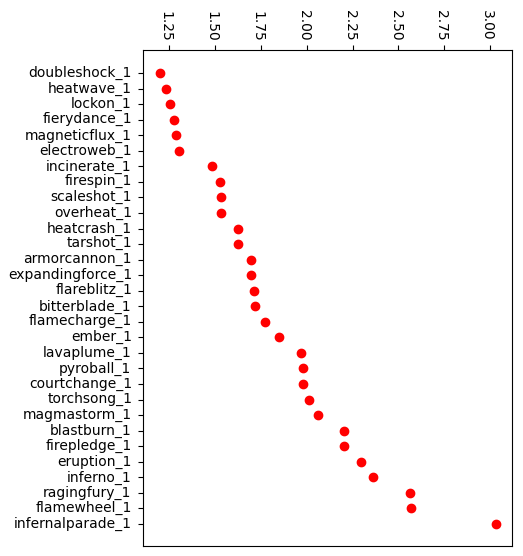
\includegraphics[width=0.4\textwidth]{top_attaques_MCA.png}
    \caption{Capacités les moins influentes (gauche), capacités les plus
    influentes (droite)}.
    \label{fig:image3}
\end{figure}

On remarque que les capacités les plus utilisées par les pokémons de type Feu
sont les attaques de type Feu (infernal parade, flame wheel, raging fury,
inferno...). Ce résultat est cohérent avec l'intuition: un pokémon a souvent
accès aux capacités de son type. Cela s'explique notamment par l'amplification
de la puissance par 50\% d'une capacité si elle est utilisée par un pokémon du
même type (mécanique appelée \textit{Same Type Attack Bonus} ou \textit{STAB}).
On remarque que les capacités les moins utilisées par les pokémons de type Feu
sont souvent de type Eau (bubble team, aqua ring, water shuriken...). Cela est
dû à deux choses: d'une part le fait que les pokémons de type Feu n'ont presque
jamais de capacités de type Eau, les deux types étant opposés; d'autre part le
fait que les pokémons de type Eau sont représentés négativement par le 3$^{e}$
axe et donc que les capacités associées à ce type y sont également représentées
négativement dans la construction de l'axe.

\subsection{Clustering des Pokémons}
Nous savons que le design des Pokémons n'a pas simplement évolué de sorte à
augmenter naïvement le total de statistiques pour les rendre strictement
meilleurs que les anciens. Nous pouvons par contre nous demander si les Pokémons
n'ont pas des archétypes de statistiques sous lesquels ils pourraient se
regrouper, et si tel est le cas, lesquels sont les plus peuplés et les plus
utilisés en stratégie (donc les plus forts) en fonction de la génération
étudiée. C'est ce qui motive l'utilisation du clustering sur les statistiques.

\subsubsection{Données utilisées et choix des clusters}
Comme expliqué précédemment, nous allons avoir besoin des données des
statistiques des Pokémons et de la génération à laquelle ils appartiennent pour
étudier les clusters par génération. Nous n'étudions que les 681 pokémons ne
pouvant pas évoluer, les autres étant moins bons que leurs évolution ils ne sont
donc pas utilisés en stratégie.

\begin{figure}[h]
    \centering
    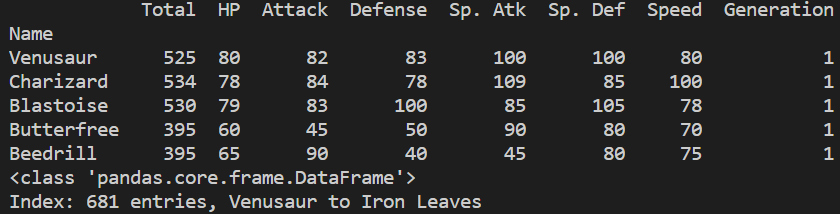
\includegraphics[width=0.8\textwidth]{Clustering/stats_gen_infos.png}
    \caption{Données utilisées pour le clustering}.
\end{figure}

Concernant le choix des clusters, nous avons affiché l'histogramme suivant,
\texttt{Figure 14}, réalisé par CAH avec la distance de Ward : 

\begin{figure}[h]
    \centering
    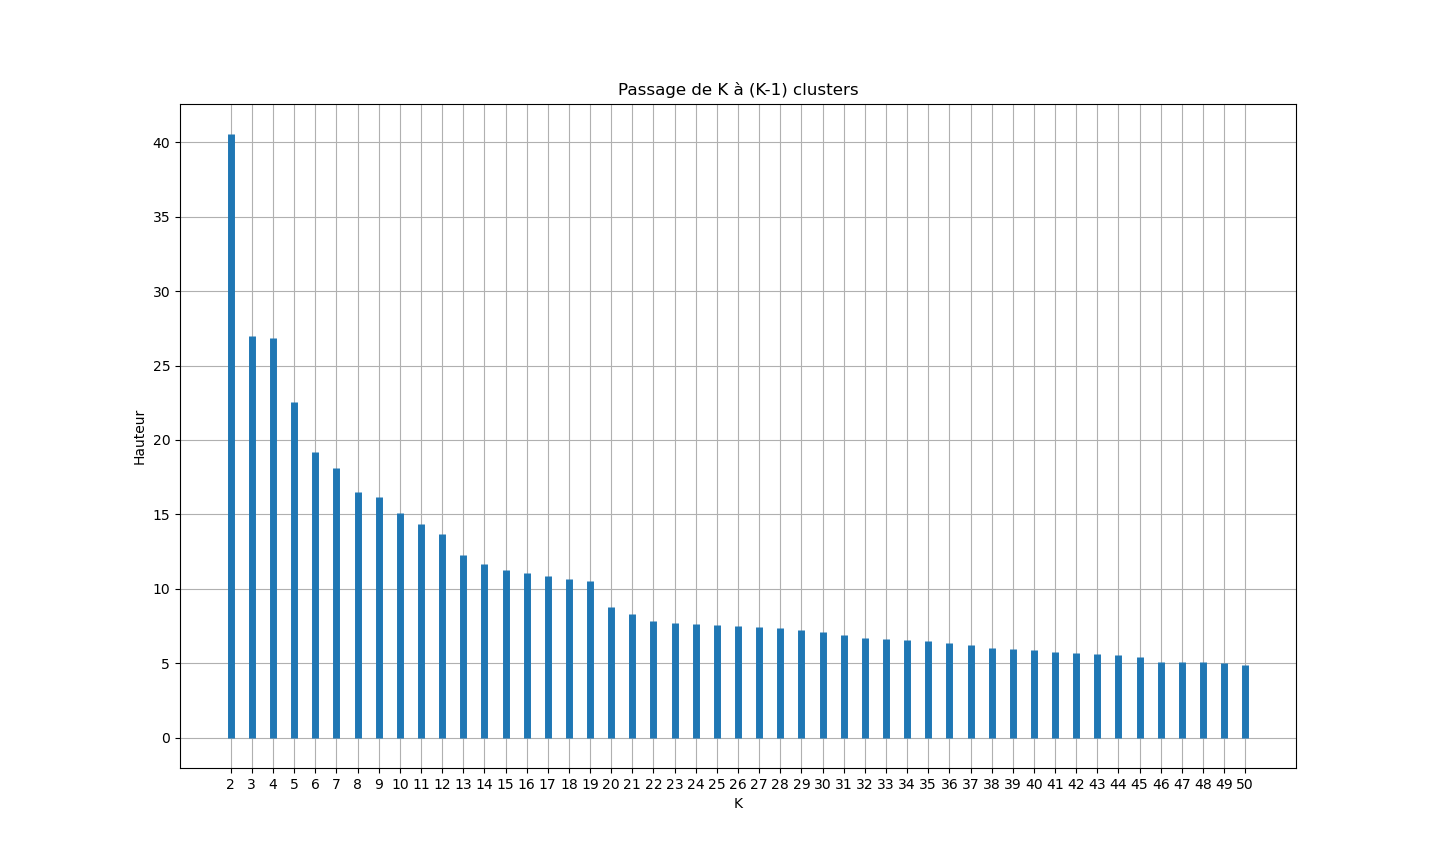
\includegraphics[width=0.7\textwidth]{Clustering/heights_k_clustering_zoomed.png}
    \caption{Gain d'inertie inter-classes lors du passage de k-1 à k classes
    ($k_max = 50$)}.
\end{figure}

Les plus gros sauts de gain sont entre 2 et 6 classes, donc il faudrait stricto
sensu prendre 2 ou 6 clusters. Cependant, les clusters obtenus ne reflétaient
que les différences en total de statistiques, ce qui est peu intéressant pour
l'étude que nous voulons mener ici. Nous avons donc choisi \textbf{k = 20
clusters}, car c'était le meilleur compromis entre trop peu de clusters et un
gros gain d'inertie inter-classes.

Ensuite, il a fallu donner du sens aux clusters obtenus. Pour cela, il suffit de
regarder la moyenne de chaque statistique des Pokémon au sein de ce cluster pour
déterminer l'archétype auquel peut être associé le cluster (quelles sont les
statistiques élevées et faibles). Voici quelques clusters observés (Fig. 15):


\begin{figure}[!h]
    \centering

    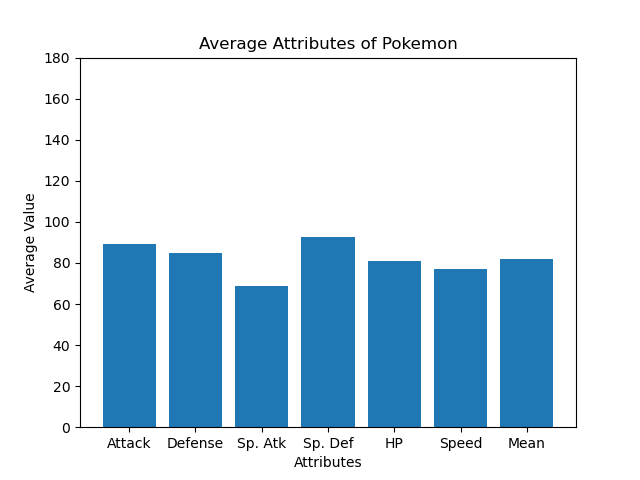
\includegraphics[width=0.3\textwidth]{Clustering/stats_cluster/7_Balanced.png}
    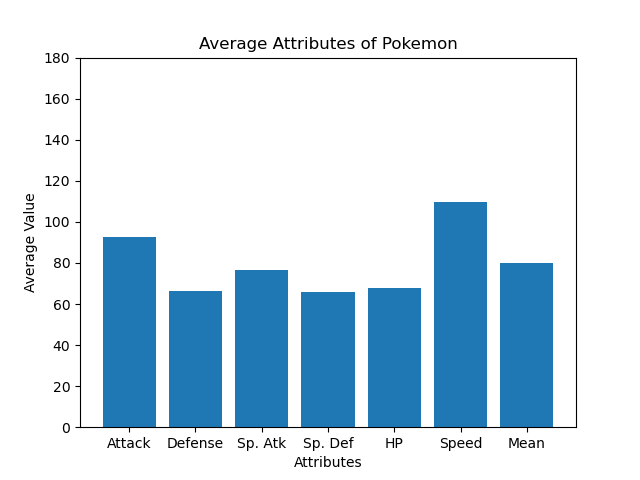
\includegraphics[width=0.3\textwidth]{Clustering/stats_cluster/10_SweepAtk.png}
    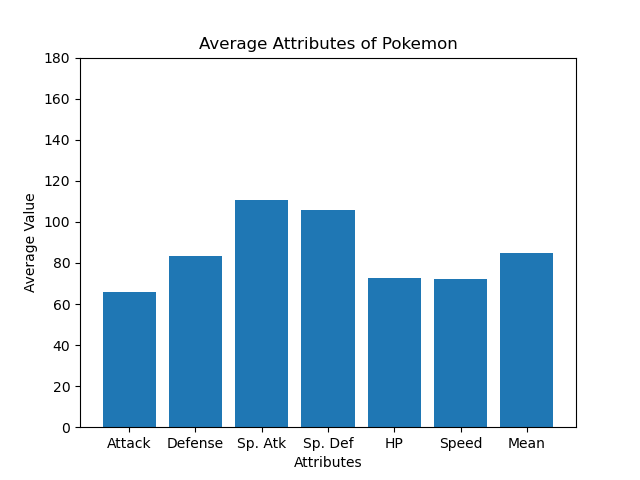
\includegraphics[width=0.3\textwidth]{Clustering/stats_cluster/8_TankSpecial.png}

    \vspace{1em}  % Ajoute un espace vertical entre les lignes

    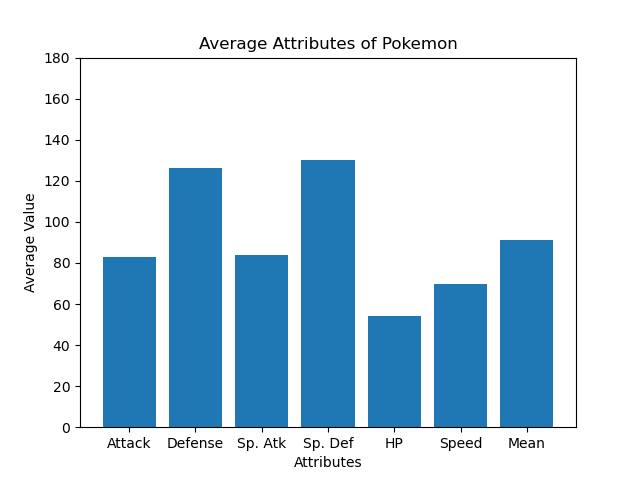
\includegraphics[width=0.3\textwidth]{Clustering/stats_cluster/9_WallMixed.png}
    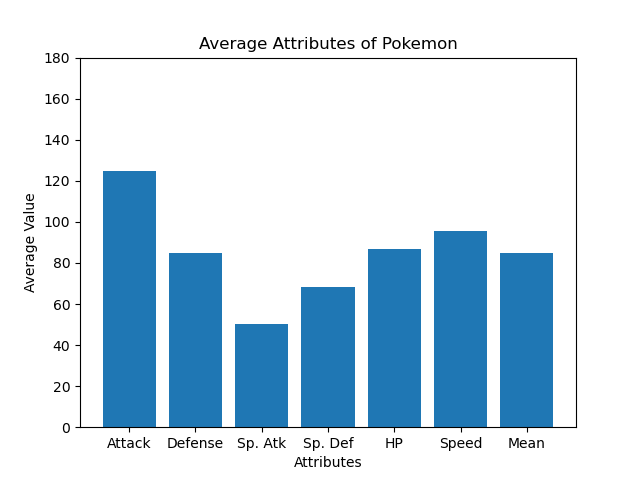
\includegraphics[width=0.3\textwidth]{Clustering/stats_cluster/14_WallbreakAtk.png}
    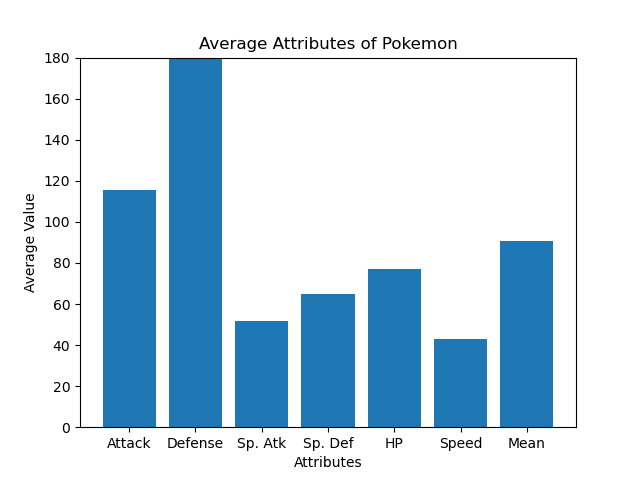
\includegraphics[width=0.3\textwidth]{Clustering/stats_cluster/16_UltraWallDef.png}

    \caption{Statistiques moyennes des Pokémon au sein de quelques clusters}
\end{figure}


\begin{enumerate}
    \item Le premier cluster comprend des Pokémon aux statistiques générales
    assez équilibrées. On l'appelle donc \textbf{Balanced}.
    \item Le deuxième cluster comprend des Pokémon aux statistiques de vitesse
    et d'attaque élevées. Ce sont des Poékmon offensifs : on les appelle
    \textbf{SweepAtk}.
    \item Le troisième comprend des Pokémon aux statistiques spéciales élevées :
    on appelle donc le cluster \textbf{TankSpecial} (un Tank peut aussi bien
    encaisser qu'asséner des coups puissants, et ici c'est sur les statistiques
    spéciales).
    \item Le quatrième cluster possède des statistiques de défense et défense
    spéciale très élevées :on l'appelle \textbf{WallMixed} (mixed car les 2
    défenses sont élevées, Wall car ce sont des Pokémon défensifs)
    \item Le cinquième cluster possède des Pokémon dont la statistique d'attaque
    est énorme : ce sont des \textbf{Wallbreak} car ils cassent les Wall.
    \item Le sixième possède une défense énorme : les Pokémon le composant
    peuvent être qualifiés de \textbf{WallDef}.
\end{enumerate}

\subsubsection{Evolution de la répartition des Pokémon au sein des clusters en fonction de leur génération}

N.B. : Les figures de cette partie sont trouvables dans l'annexe en fin de
document.

Nous allons maintenant nous atteler à la répartition des Pokémon au sein des
clusters, pour comprendre les changements de design (= choix des archétypes
dominants) au fil des générations. Pour cela, nous avons calculé pour chaque
génération la part du nombre de Pokémon dans chaque cluster. Les résultats sont
affichés Figure \ref{fig:annexe1}, par ordre croissant de génération (de la plus
ancienne à la plus récente.



\begin{itemize}
    \item La première génération met l'accent sur les Pokémon Balanced et Sweep.
    C'est donc une génération assez équilibrée et offensive.
    \item La seconde introduit beaucoup de Pokémon Balanced et WeakBalanced
    (Balanced mais avec un total plus faible), l'équilibre des statistiques est
    une caractéristique forte de cette génération.
    \item La troisième introduit énormément de WeakBalanced, on continue sur la
    lignée des Pokémon équilibrés mais plus faibles.
    
On peut donc remarquer que les 3 premières générations sont surtout à dominante
équilibrée.
    \item Dès la quatrième génération, on observe une réduction de la proportion
    de Pokémon équilibrés au profit des TankSpecial, LegendaryOffensive et
    MixedAttacker. Les Legendary sont des Pokémon au total de statistiques plus
    élevées, donc on remarque que le total de statistiques augmente et que les
    Pokémon deviennt de plus en plus orientés sur l'offensive.
    \item La cinquième génération exacerbe encore plus cette spécialisation
    offensive avec un fort taux de SweepAtk, 600BSTAtk, TankPhysical.
    \item La sixième génération est marquée par une explosion du nombre de
    LegendaryOffensive, SweepSpA et 600BSTAtk. Elle est donc encore plus
    offensive que jamais, avec en plus le total de statistiques moyen le plus
    élevé encore à ce jour.

Les générations 4 à 6 sont donc extrêmement offensives.
    \item La septième génération offre un panel de Pokémon TankPhysical élevé
    mais aussi un grand taux de Pokémon défensifs (Wall, Tank, Fat). C'est une
    génération défensive, ce qui permet de compenser la domination des Pokémon
    offensifs introduits lors des 3 générations précédentes.
    \item La huitième génération reprend une tendance assez offensive, avec
    beaucoup de Pokémon Attacker, Wallbreak, Sweep.
    \item La neuvième génération aussi, mais à dominante un peu plus équilibrée
    (augmentation de la proportion de Tank).
\end{itemize}

Les générations 7 à 9 semblent avoir une cohérence : elles introduisent des
Pokémon à archétypes toujours plus originaux et en fonction des Pokémon passés
pour équilibrer les archétypes.

\subsubsection{Evolution des usages au sein des différents clusters en fonction de la génération}

Nous avons vu quels étaient les choix de design privilégiés en fonction des
générations. Nous allons maintenant voir quels sont les plus utilisés/efficaces
en stratégie.


\begin{itemize}
    \item La première génération est marquée par des Pokémon à hautes
    statistiques orientées sur l'attaque et le special en tant que principaux
    représentants en stratégie, malgré l'emphase de design sur les statistiques
    équilibrées. Cela montre que le design équilibré n'est pas le plus viable de
    nos jours.
    \item Les meilleurs Pokémon de deuxième, troisième et quatrième génération
    sont des Pokémon défensifs (Blissey, FatMixedHP, WallDef) avec des
    statistiques extrêmes (Blissey a la plus haute statistique de HP du jeu).
    Encore une fois, l'archétype le plus peuplé n'est pas le plus populaire, et
    seuls les Pokémon extrêmes se démarquent.
    \item En cinquième génération, on a un usage élevé pour les Pokémon très
    offensifs (600BSTAtk, MixedSweeper) et très défensifs (BlisseyLike,
    FatMixedHP). Cependant, la versatilité dans le domaine de prédilection
    semble être importante (Mixed signifiant posséder autant d'attaque que
    d'attaque spéciale, ou autant de défense que de défense spéciale).
    L'imprévisibilité d'un Pokémon, sa capacité à être efficace de manière
    offensive ou défensive sur le spectre physique ou spécial semble être un
    facteur important.
    \item La génération 6 est marquée par une absence quasi totale du paysage
    stratégique actuel. Cela s'explique car la mécanique principale (donner une
    nouvelle forme avec des statistiques Legendary à des Pokémon existants) a
    disparu dans la génération actuelle, donc ses Pokémon les plus puissants
    n'apparaissent pas dans les données d'usage.
    \item La 7ème génération voit le taux d'usage des Pokémon WallMixed exploser
    (défensifs et versatiles) ainsi qu'un haut taux de MixedSweeper (rapide et
    avec une haute attaque et attaque spéciale). Là encore, la spécialisation
    dans un domaine (offensif ou défensif) avec de la versatilité semble être
    importante.
    \item La génération 8 poursuit la tendance à favoriser les Pokémon
    versatiles qui excellent dans un des deux domaines, cette fois en favorisant
    les Pokémon offensifs. On observe aussi une explosion de l'usage moyen des
    Pokémon en général : encore une preuve du powercreep.
    \item Enfin, la neuvième génération voit le profil Tank (beaucoup d'attaque
    et de défense, ou beaucoup d'attaque et de défense spéciale) grimper en
    flèche. Il semble intéressant d'être capable de frapper fort en encaissant
    bien les coups, même au détriment de la vitesse (plutôt que simplement
    frapper vite et fort).
    
\end{itemize}

En résumé, nous avons vu que les taux de répartition dans les clusters (donc la
"mode" de design associée à la génération) n'est pas corrélée à la viabilité de
ces Pokémon. Il faut remplir un rôle spécifique, avec des statistiques
spécialisées et optimisées pour remplir ce rôle. C'est pourquoi l'archétype
Balanced, très largement peuplé par les Pokémon des premières générations, n'est
pas viable dans la génération actuelle et semble avoir été délaissé petit à
petit au profit de Pokémon offensifs et défensifs, qu'ils soient lents ou
rapides. La popularité de la versatilité dans les générations pourrait remettre
en cause notre hypothèse de base de la spécialisation toujours plus pointue des
Pokémon pour qu'ils deviennent plus puissants. Cependant, les statistiques ne
font pas tout : les Pokémon les plus joués ne le sont pas que grâce à leurs
statistiques, mais leurs capacités, talents et types pèsent extrêmement lourd
dans la balance. On peut penser à Kingambit et Great Tusk, qui sont 2 des
Pokémon les plus joués actuellement et qui ont un profil Tank, mais qui le sont
surtout pour leurs capacités (et leur talent pour Kingambit) qui les aide
grandement à accomplir leur rôle.

\section{Conclusion et pistes d'amélioration}

Nous avons pu voir que le powercreep existe bel et bien dans les jeux Pokémon.
Cependant, il ne s'agit pas d'une simple évolution à la hausse des statistques
des pokémons (comme peut le faire par exemple le jeu de carte à jouer Pokémon
TCG, pour lequel le powercreep est un fort argument marketing). Il n'est
également pas évident que les pokémons sont de plus en plus spécialisés, comme
nous avons pu le voir lors de l'étude de la variante inter-statistiques.

En revanche, certains choix de design comme peuvent expliquer plus subtilement
les changements de viabilité. L'ACP a permis de montrer que les statistiques,
sans être corréler entre elles, suivent tout de même certaines tendances. L'ACM
sur les capacités a pu montrer que le choix d'un type conditionne certains
pokémons au-delà des simples résistances et faiblesses du type via la notion de
coverage.

Enfin, nous avons vu qu'une partie de la viabilité des pokémons peut s'expliquer
par les choix d'archétypes qui leur sont faits et que nous avons pu déterminer
lors du clustering : certains archétypes particulièrement efficaces sont
également particulièrement peuplés par des pokémons des dernières générations
Ainsi, la viabilité des pokémons plus récent est en partie due à leur
appartenance à de meilleurs archétypes.

D'autres facteurs qui ne rentraient pas dans le cadre de notre étude pourraient expliquer la viabilité des pokémons.
L'influence des talents n'est pas quantifiable statistiquement, car de trop nombreux talents
sont uniques à une espèce de pokémon : on ne peut alors pas dissocier la
viabilité du pokémon à celle du talent. C'est pourtant une partie importante de
la viabilité de certains pokémons (Kingambit, Gholdengo...). De même, les objets
n'ont pas été pris en compte : ceux-ci sont utilisables par n'importe quels
pokémons, mais certains en bénéficient plus que d'autres. Si l'introduction de
nouveaux objets influants est assez rare (raison pour laquel nous les avons exclu
de notre étude), l'objet \textit{Grosses Bottes} en génération 8 a grandement
modifié la viabilité de certains pokémons et mériterait à lui seul une étude
similaire à celle-ci. Enfin, la notion de \textit{metagame} n'a pas été prise en compte : un pokémon peut être fort car il est une bonne réponse à d'autres pokémons (comme Great Tusk). Il y a donc des facteurs extérieurs aux pokémons eux-mêmes qui influent sur leur viabilité.
\newpage
\section{Annexe}

\begin{figure}[!h]
    \centering

    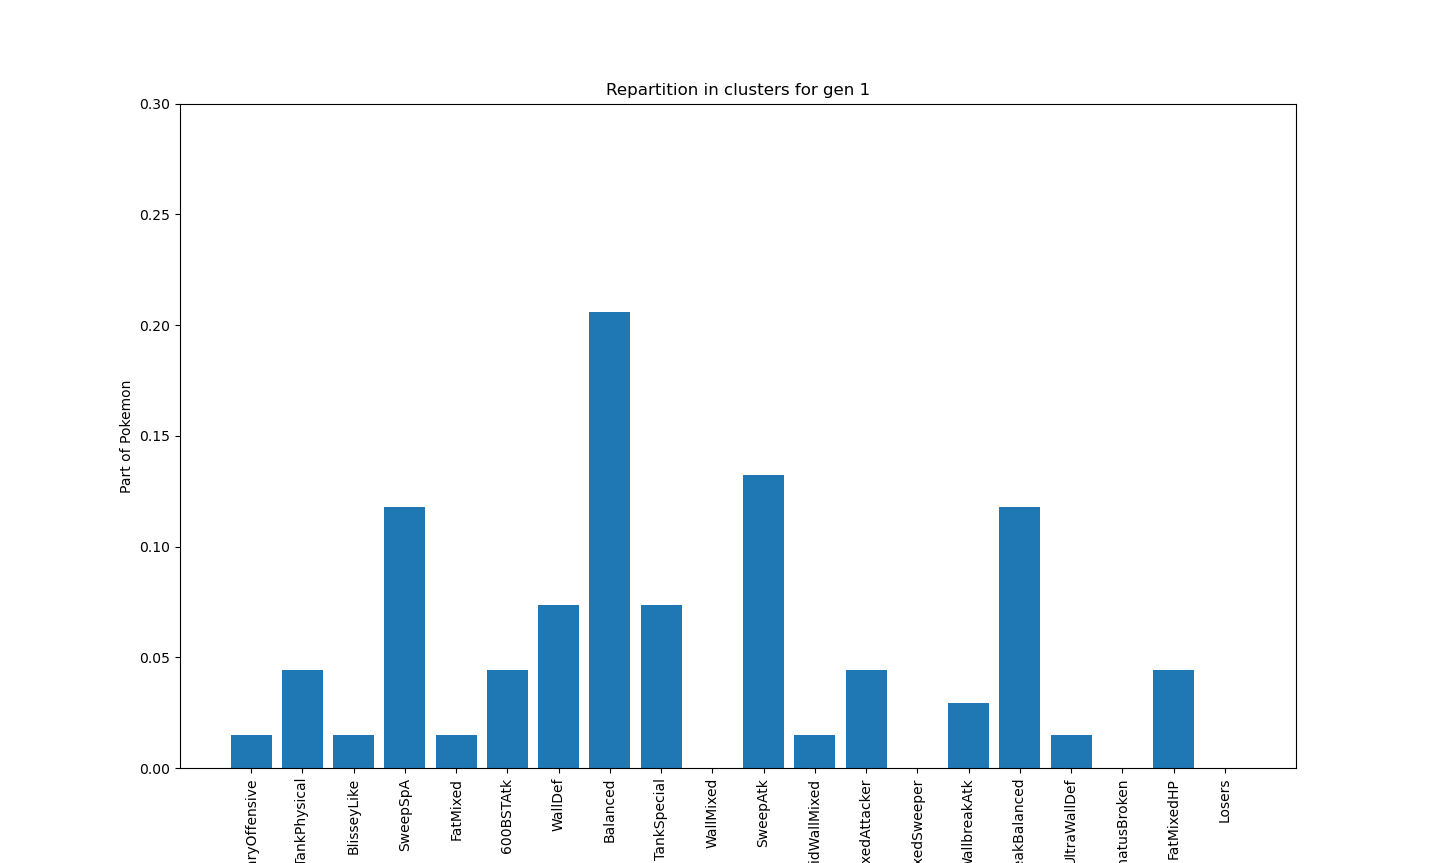
\includegraphics[width=0.4\textwidth]{Clustering/number_poke_gen/gen1.png}
    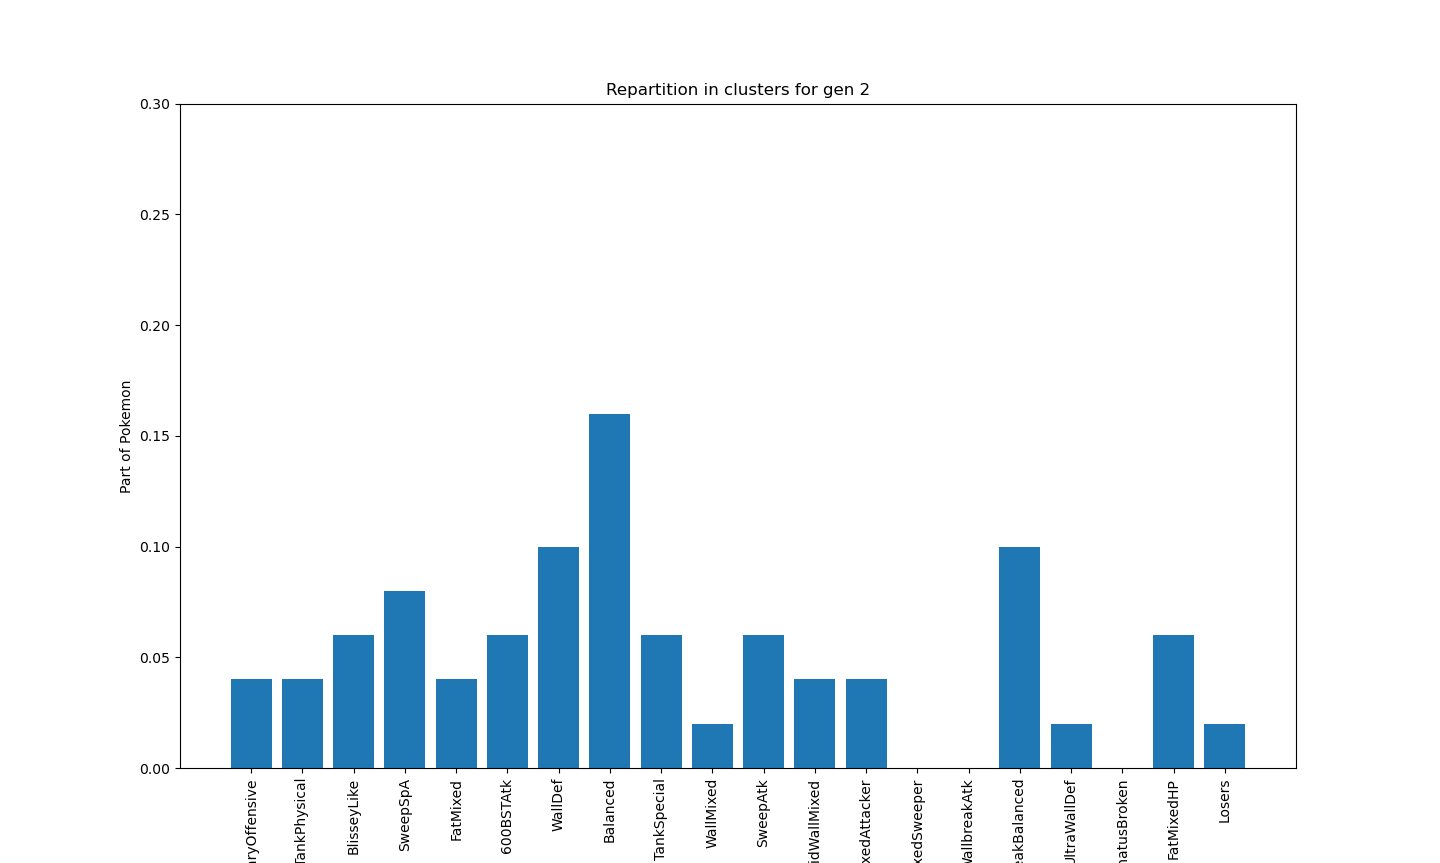
\includegraphics[width=0.4\textwidth]{Clustering/number_poke_gen/gen2.png}
    

    \vspace{1em}  % Ajoute un espace vertical entre les lignes

    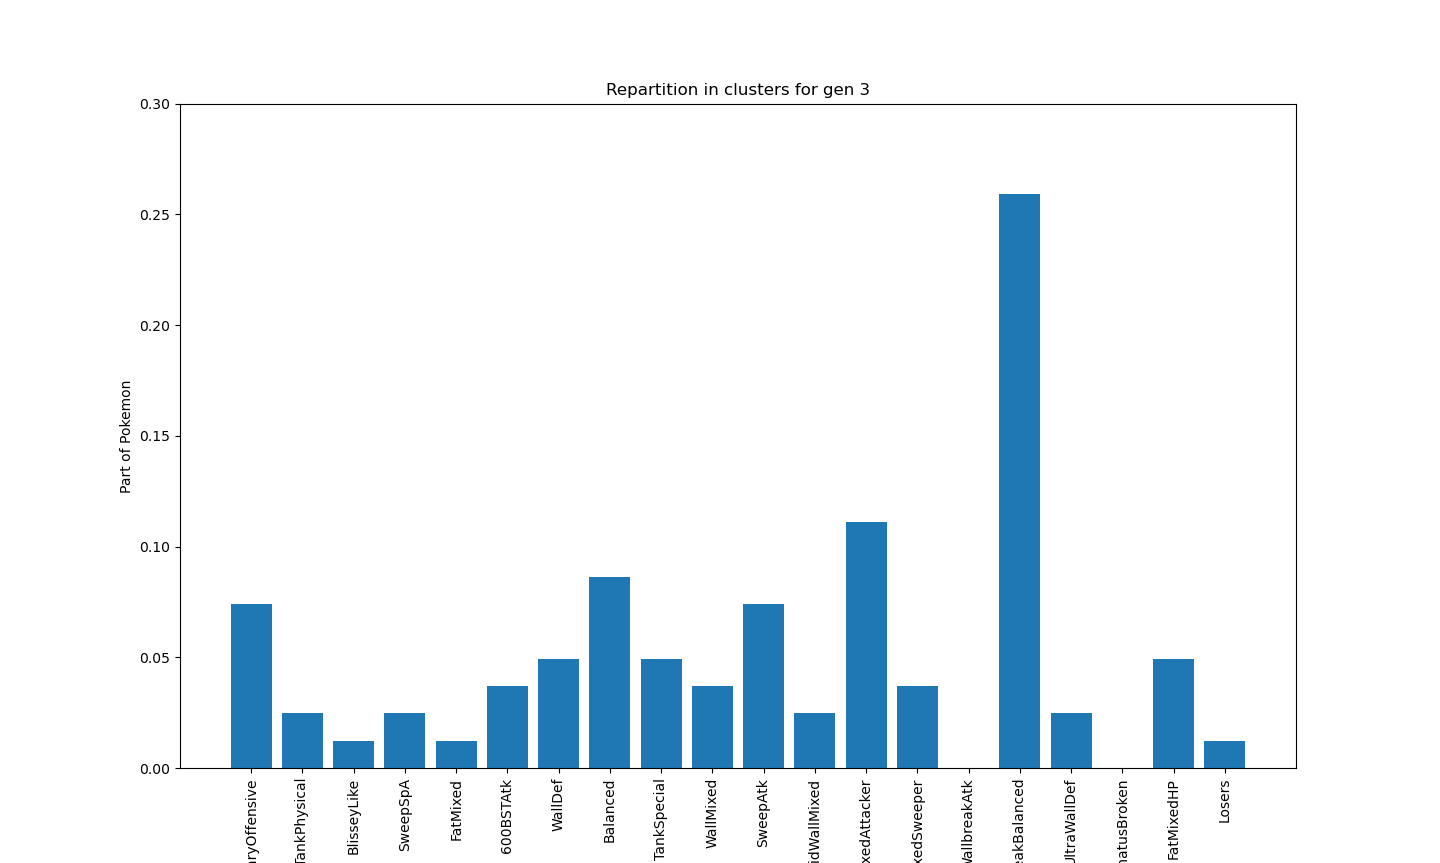
\includegraphics[width=0.4\textwidth]{Clustering/number_poke_gen/gen3.png}
    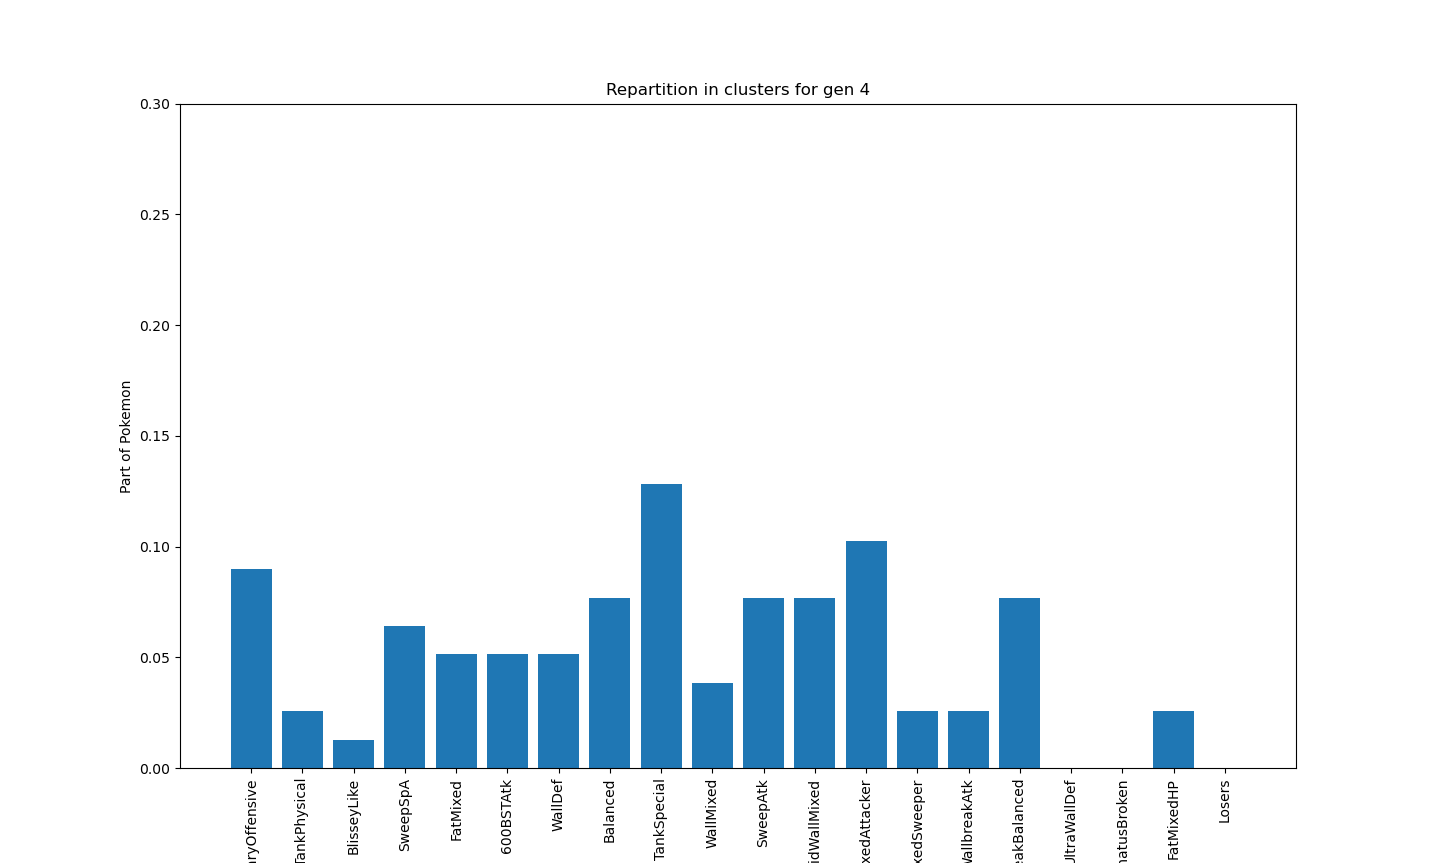
\includegraphics[width=0.4\textwidth]{Clustering/number_poke_gen/gen4.png}
    

    \vspace{1em}  % Ajoute un espace vertical entre les lignes

    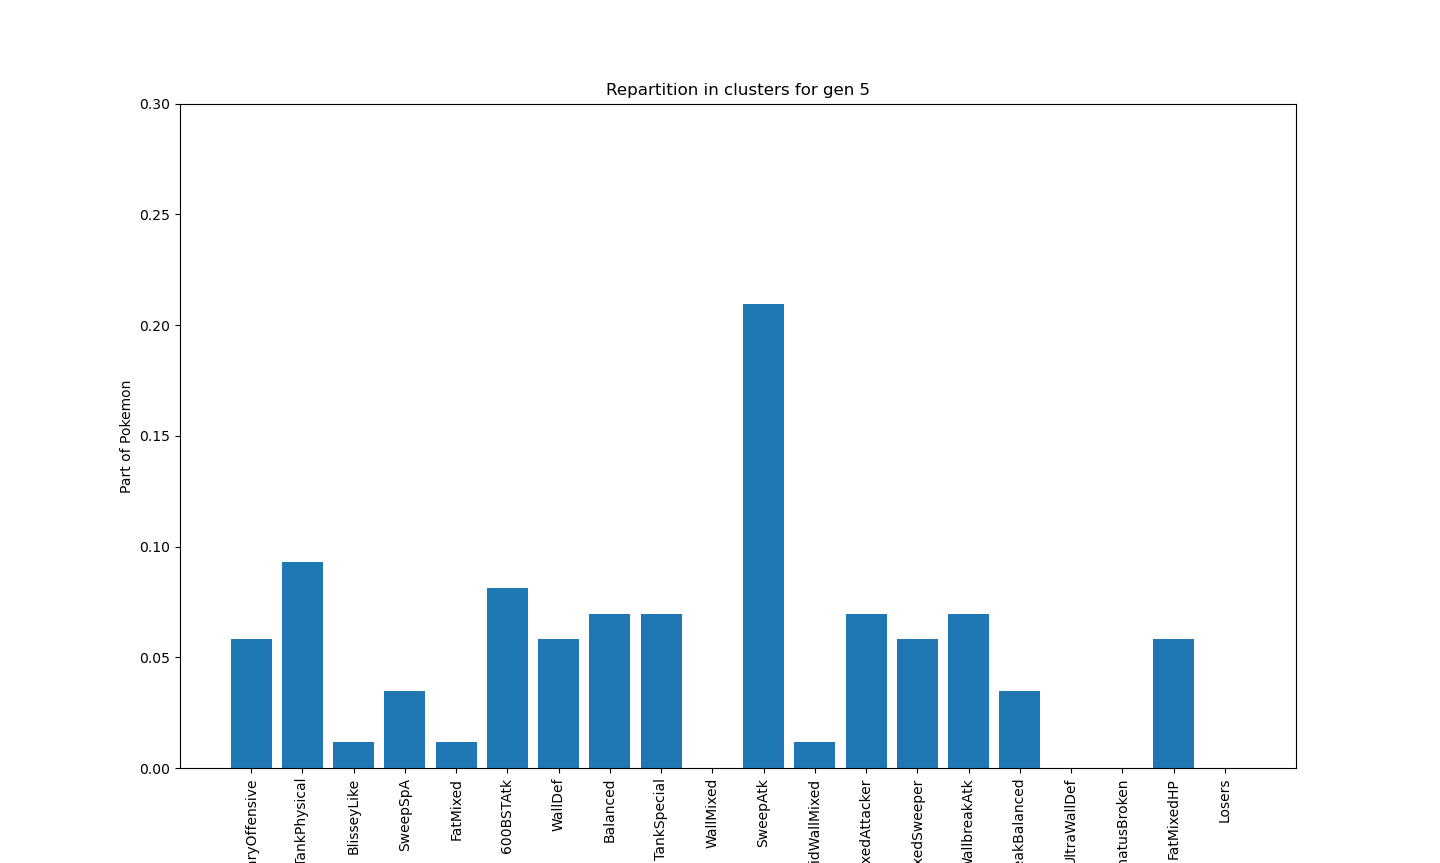
\includegraphics[width=0.4\textwidth]{Clustering/number_poke_gen/gen5.png}
    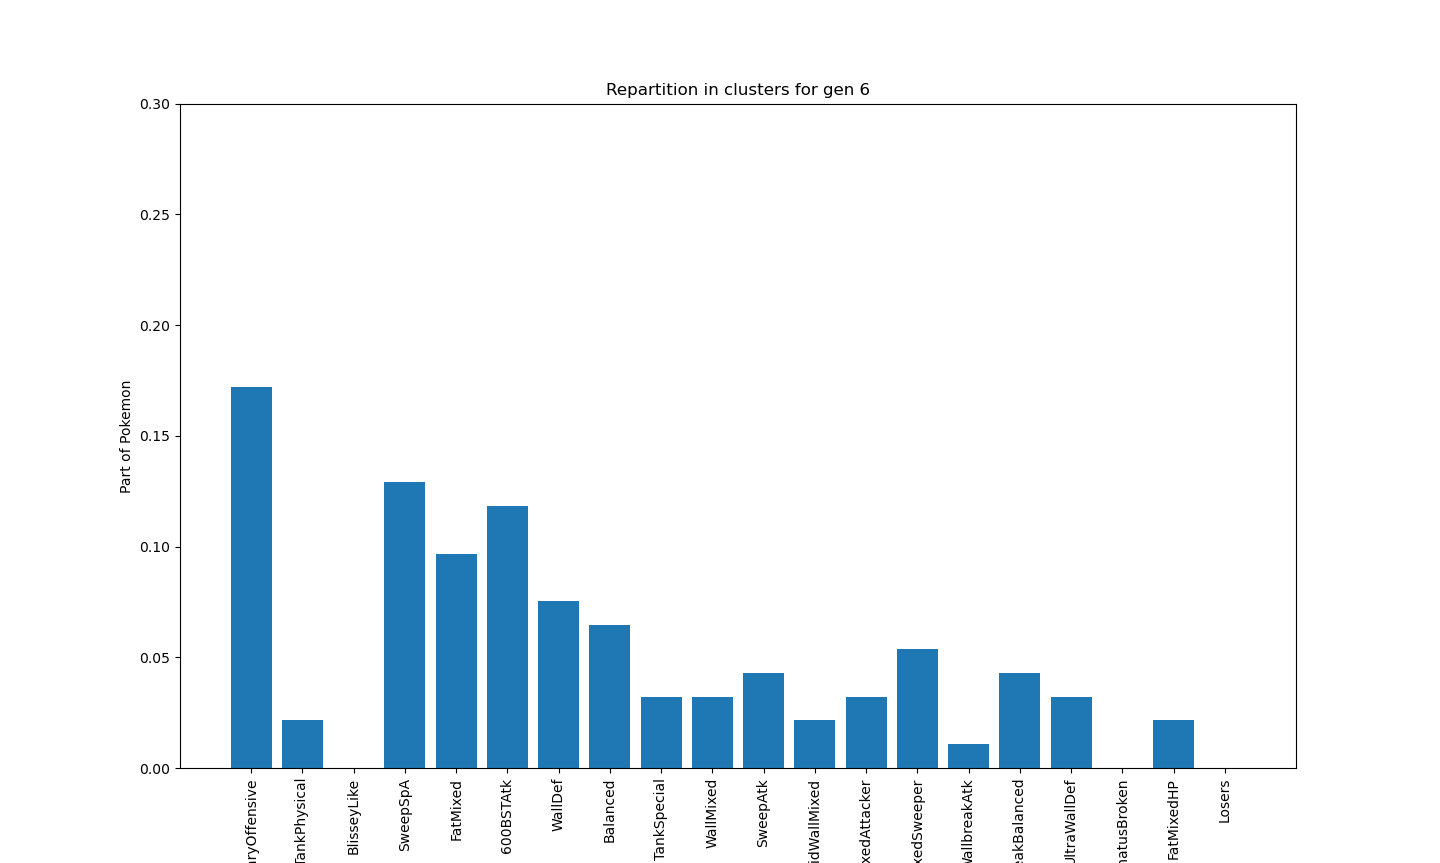
\includegraphics[width=0.4\textwidth]{Clustering/number_poke_gen/gen6.png}
    

    \vspace{1em}  % Ajoute un espace vertical entre les lignes

    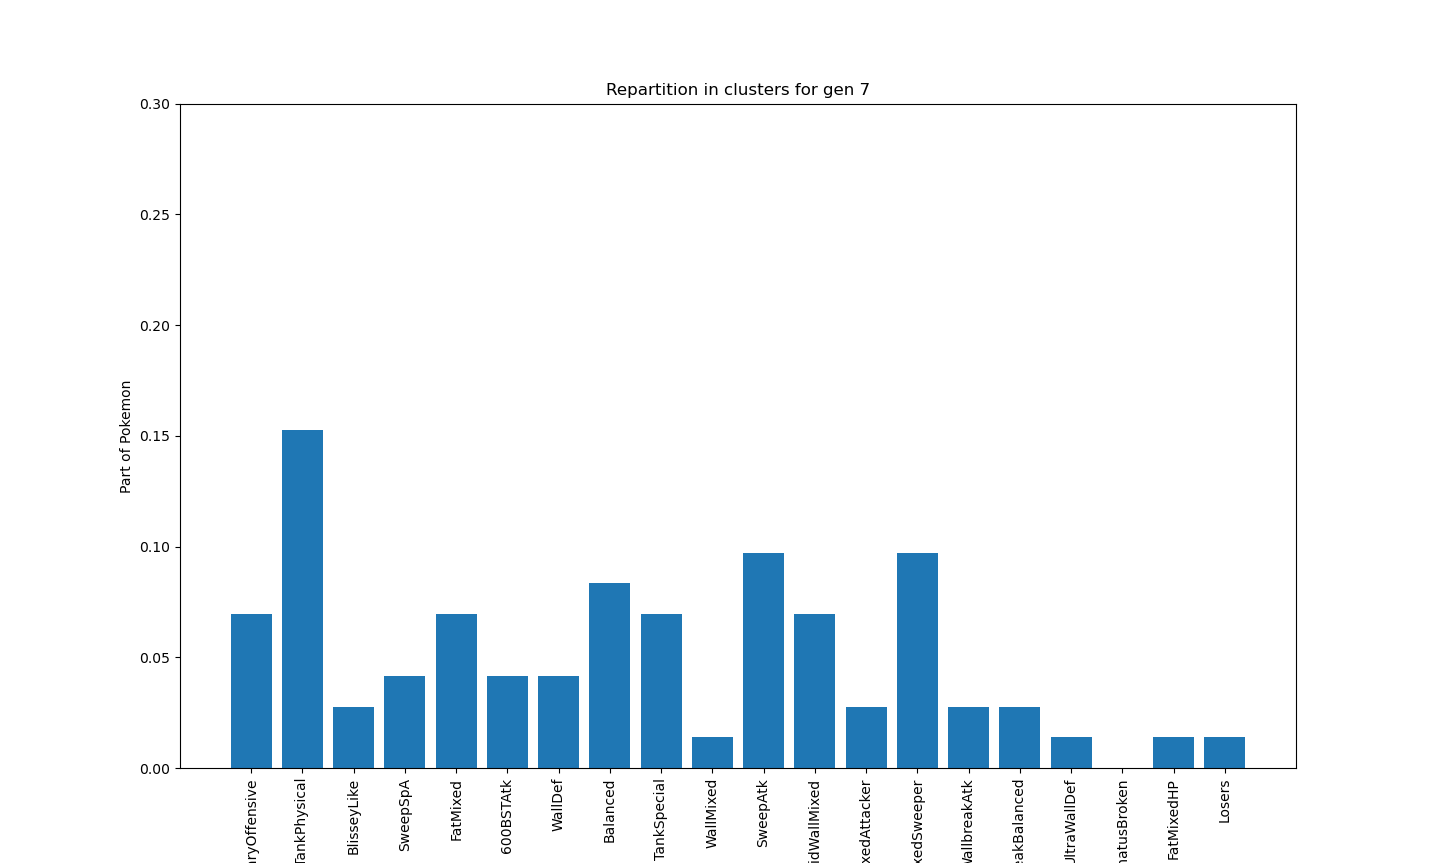
\includegraphics[width=0.4\textwidth]{Clustering/number_poke_gen/gen7.png}
    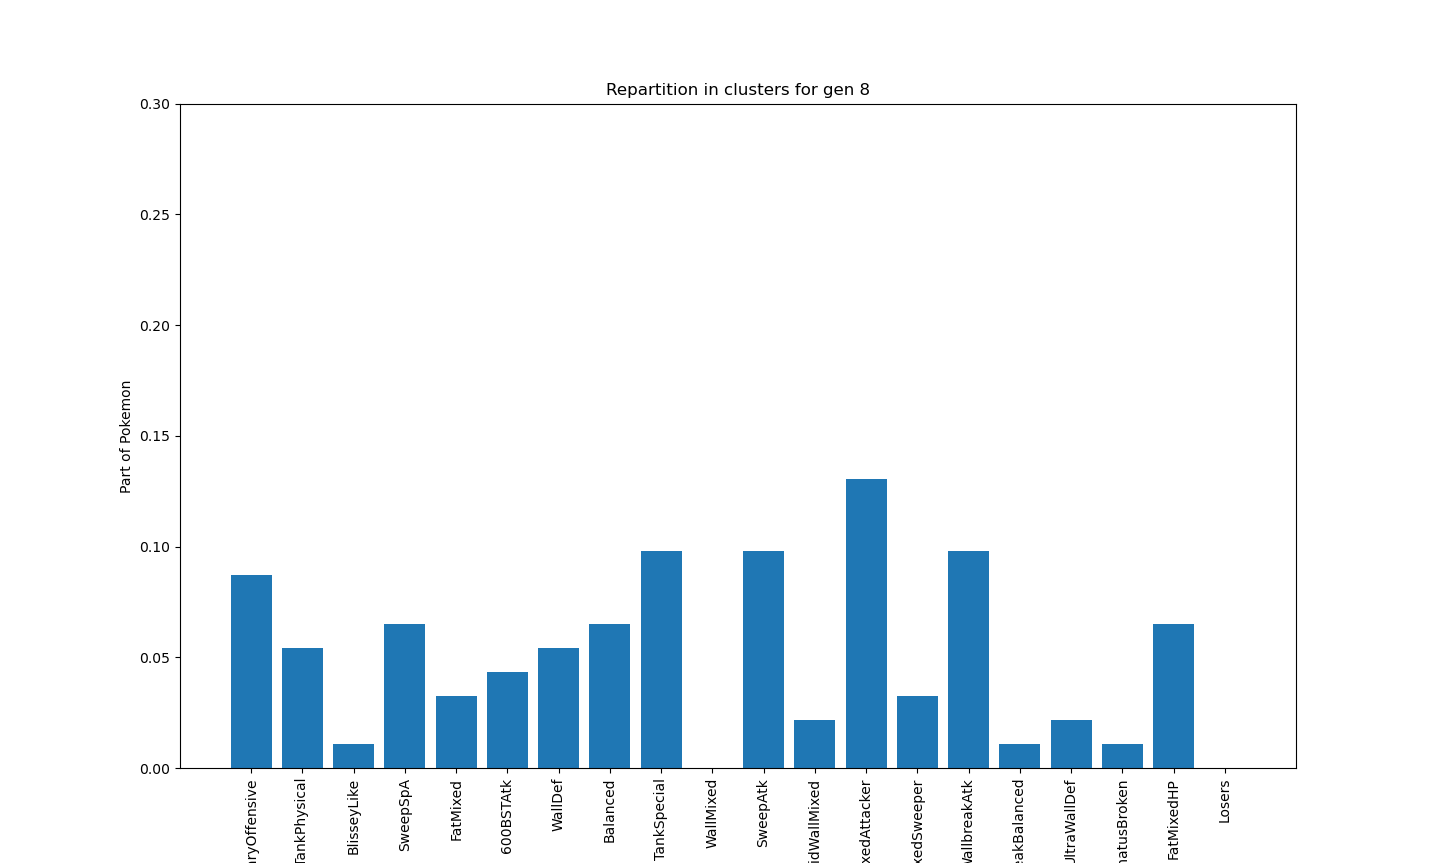
\includegraphics[width=0.4\textwidth]{Clustering/number_poke_gen/gen8.png}
    

    \vspace{1em}  % Ajoute un espace vertical entre les lignes

    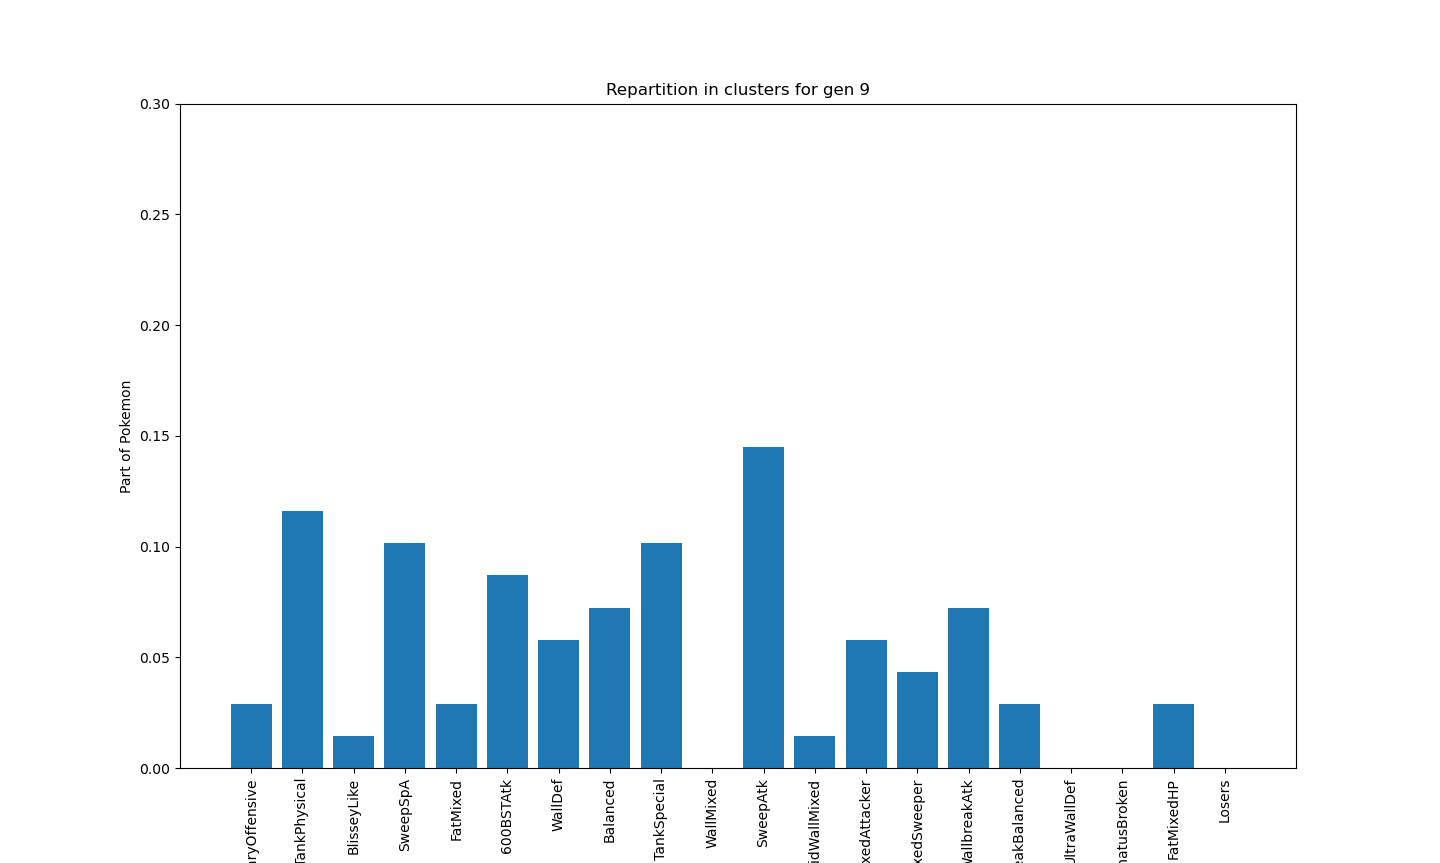
\includegraphics[width=0.4\textwidth]{Clustering/number_poke_gen/gen9.png}
    \caption{Répartition des Pokémon au sein des clusters}
    \label{fig:annexe1} % Add a proper reference to the \label command
\end{figure}

\begin{figure}[!h]
    \centering

    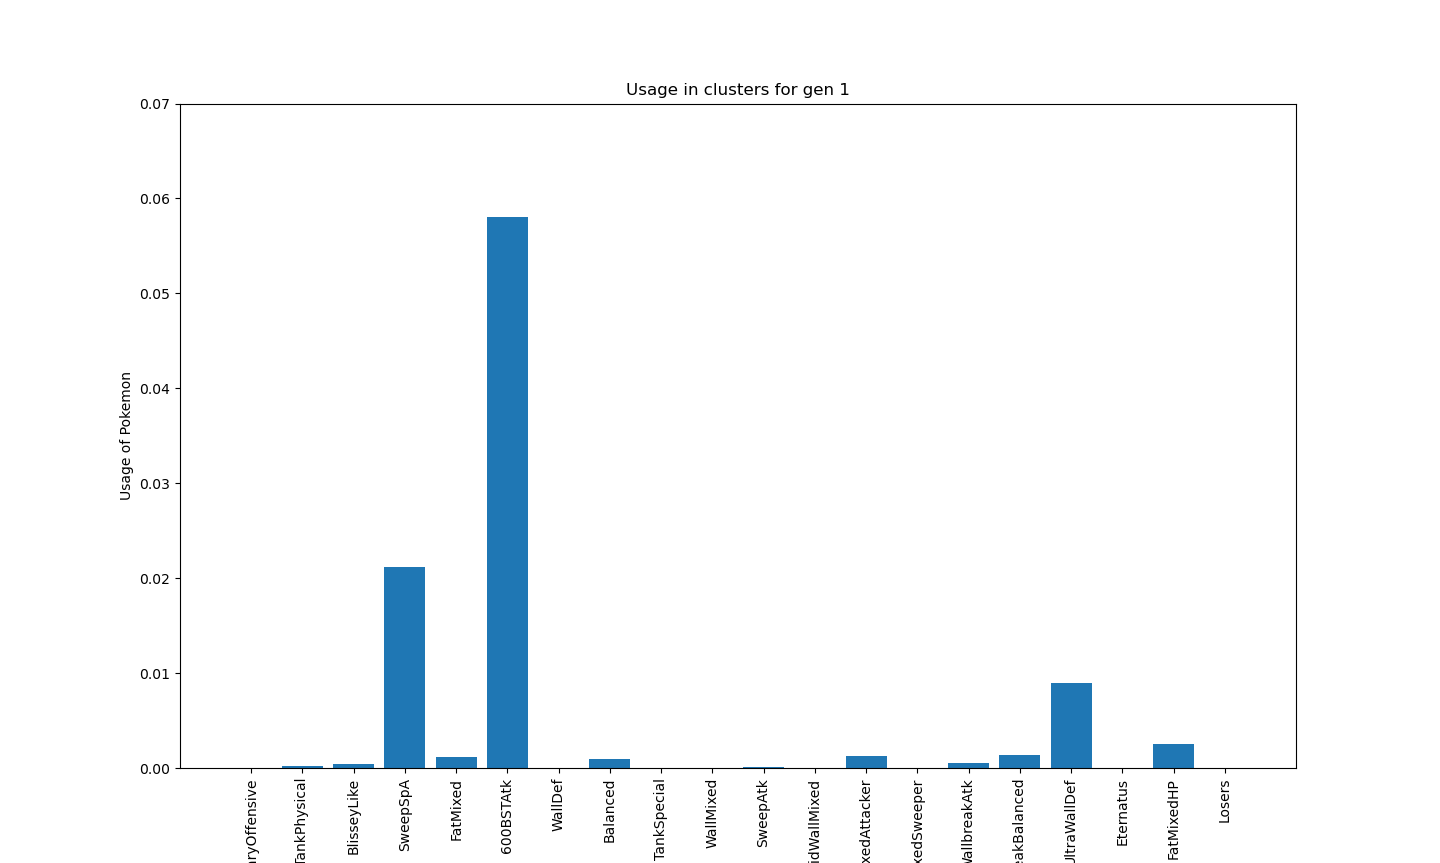
\includegraphics[width=0.45\textwidth]{Clustering/usage_gen/gen1.png}
    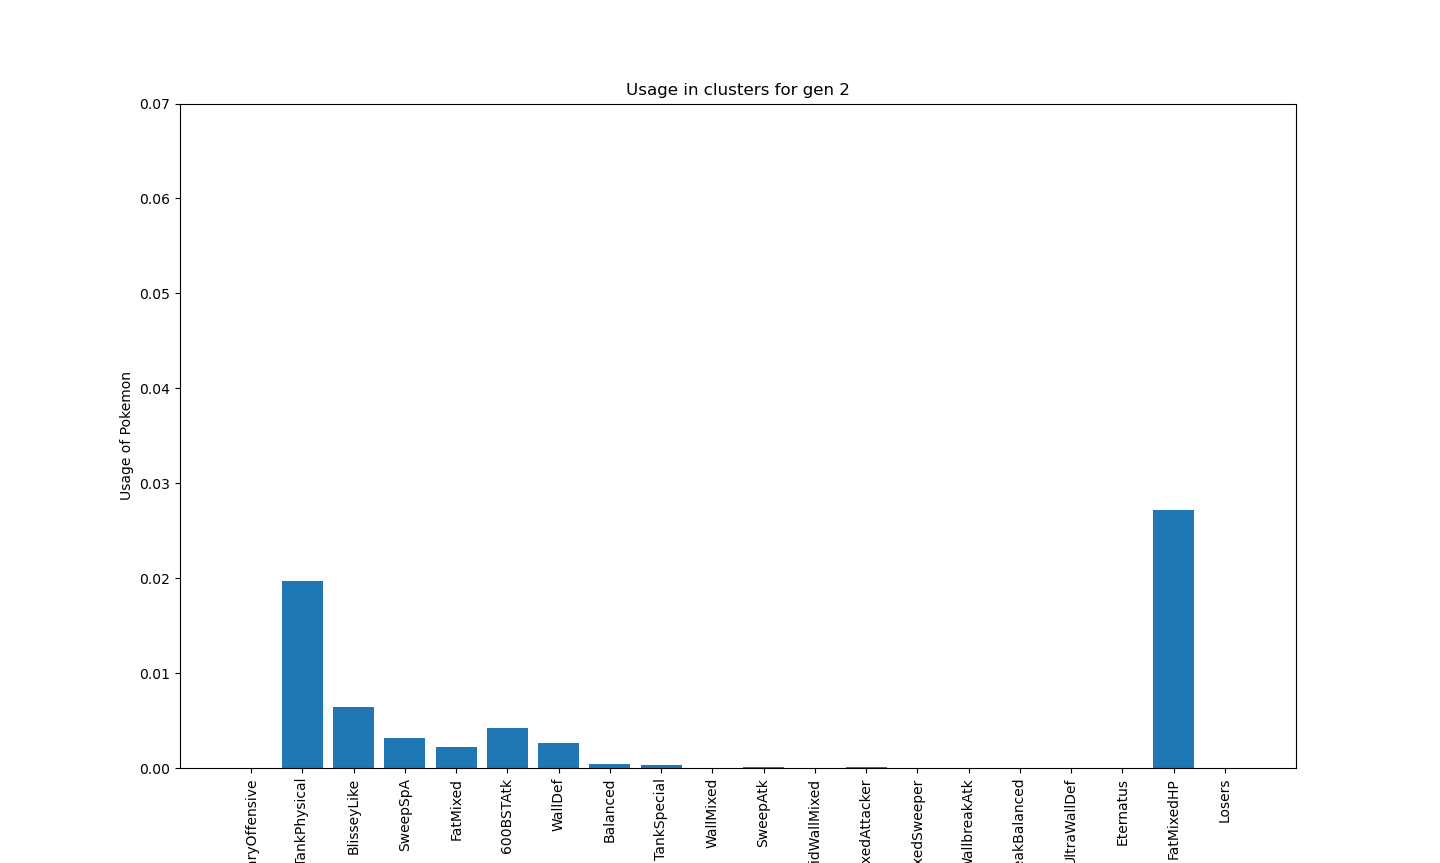
\includegraphics[width=0.45\textwidth]{Clustering/usage_gen/gen2.png}
    

    \vspace{1em}  % Ajoute un espace vertical entre les lignes

    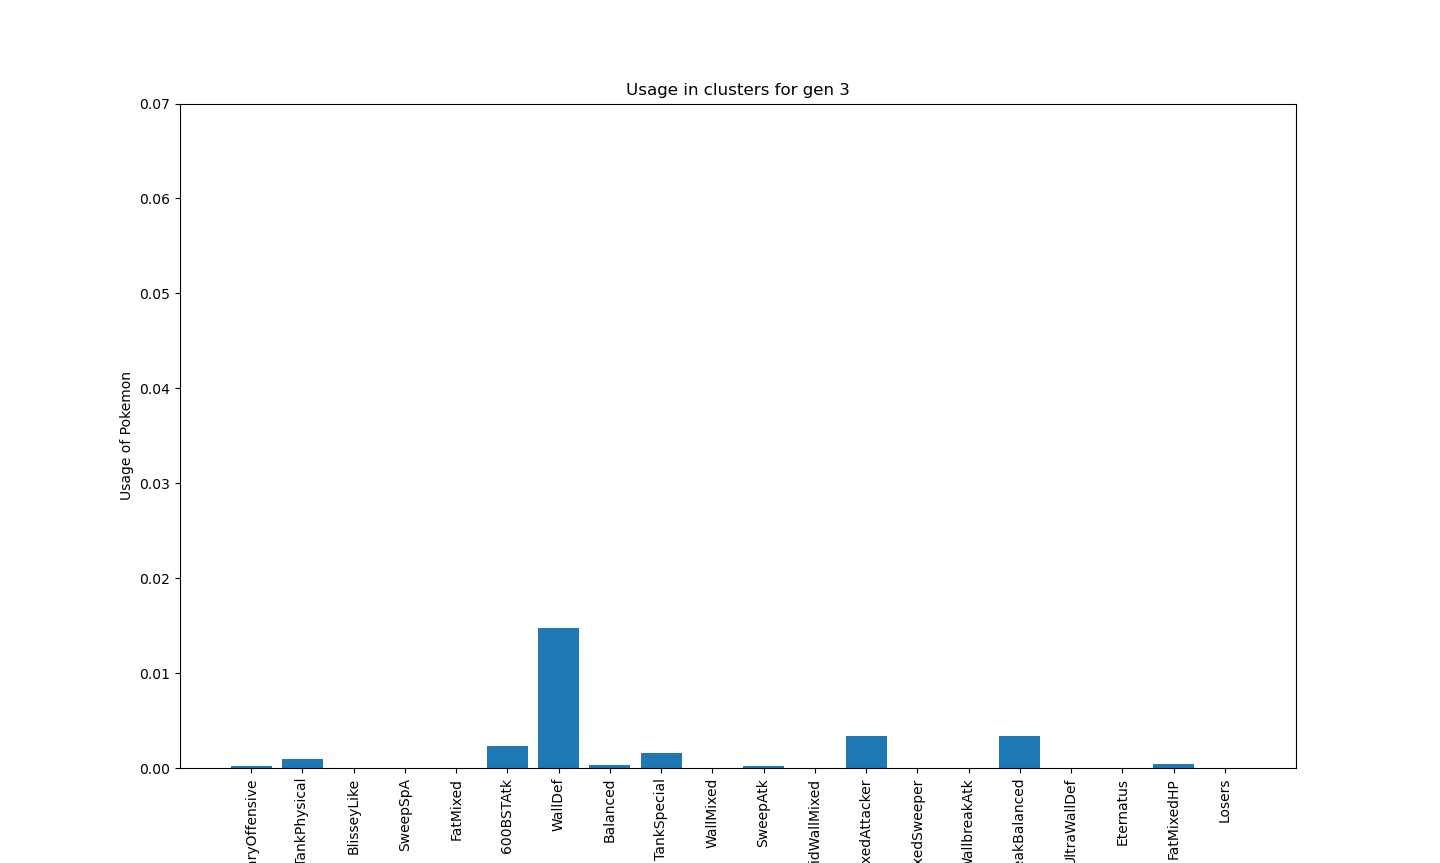
\includegraphics[width=0.45\textwidth]{Clustering/usage_gen/gen3.png}
    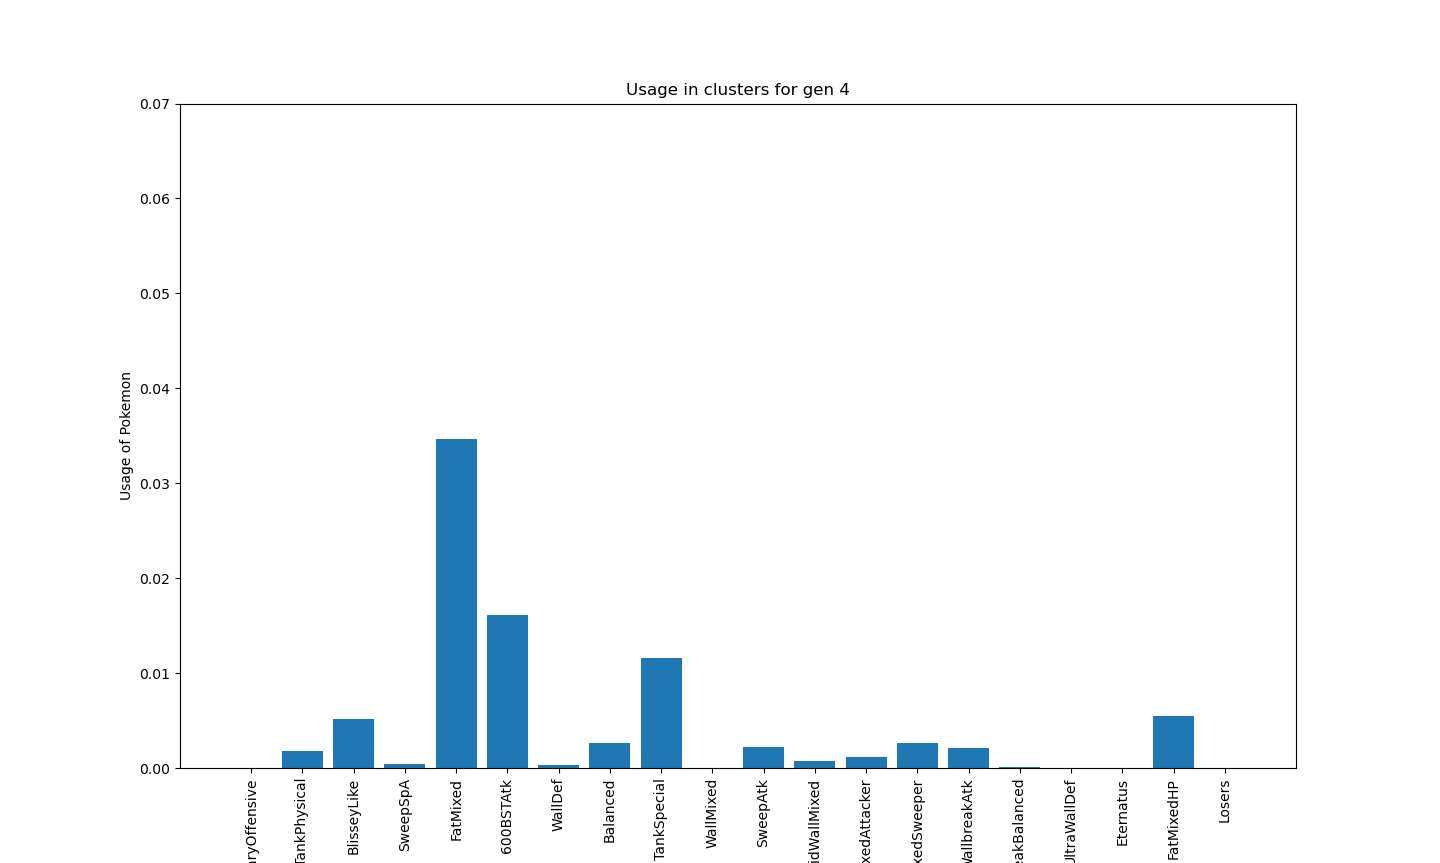
\includegraphics[width=0.45\textwidth]{Clustering/usage_gen/gen4.png}
    

    \vspace{1em}  % Ajoute un espace vertical entre les lignes

    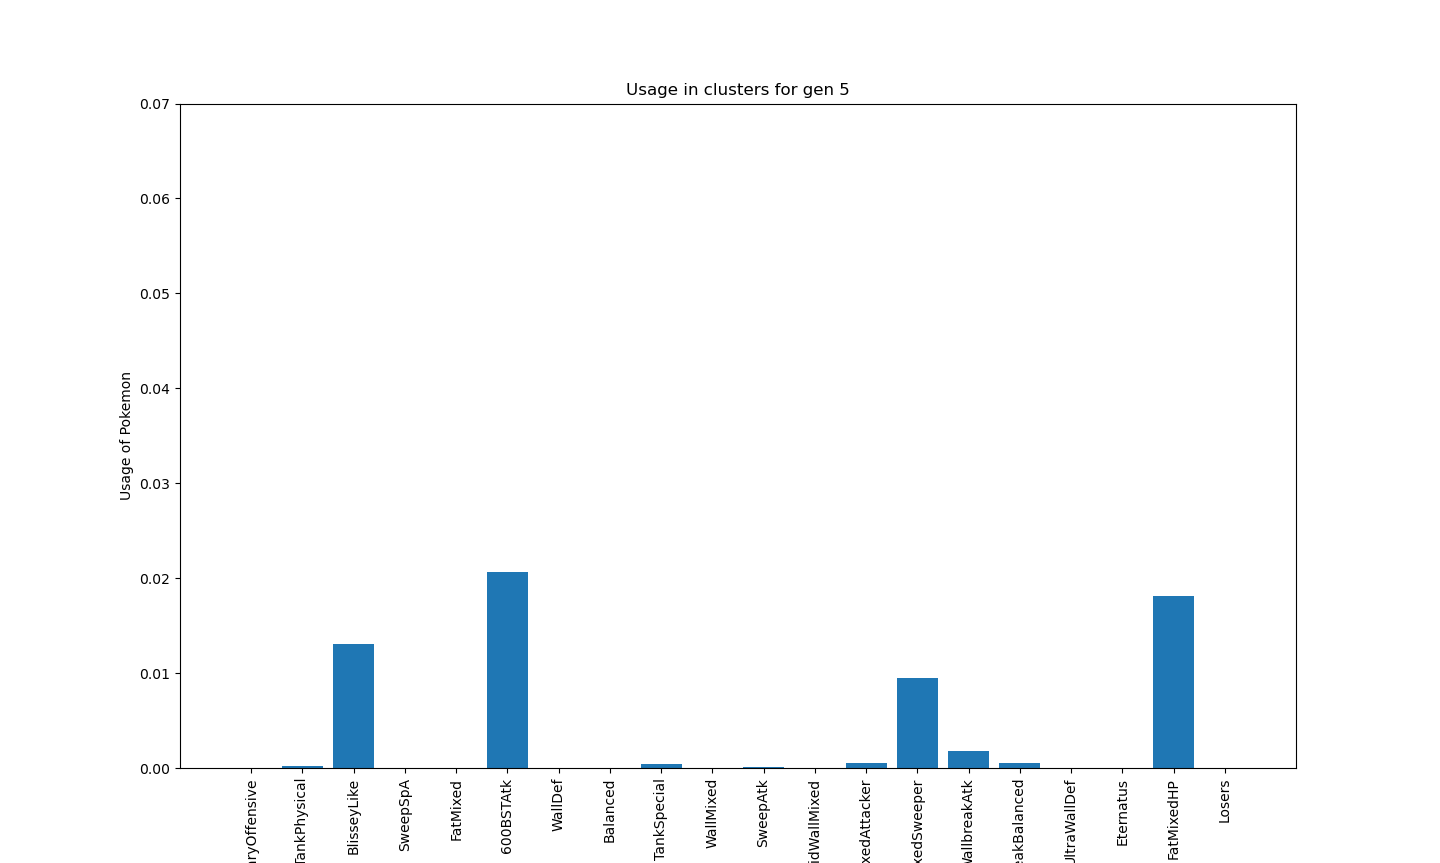
\includegraphics[width=0.45\textwidth]{Clustering/usage_gen/gen5.png}
    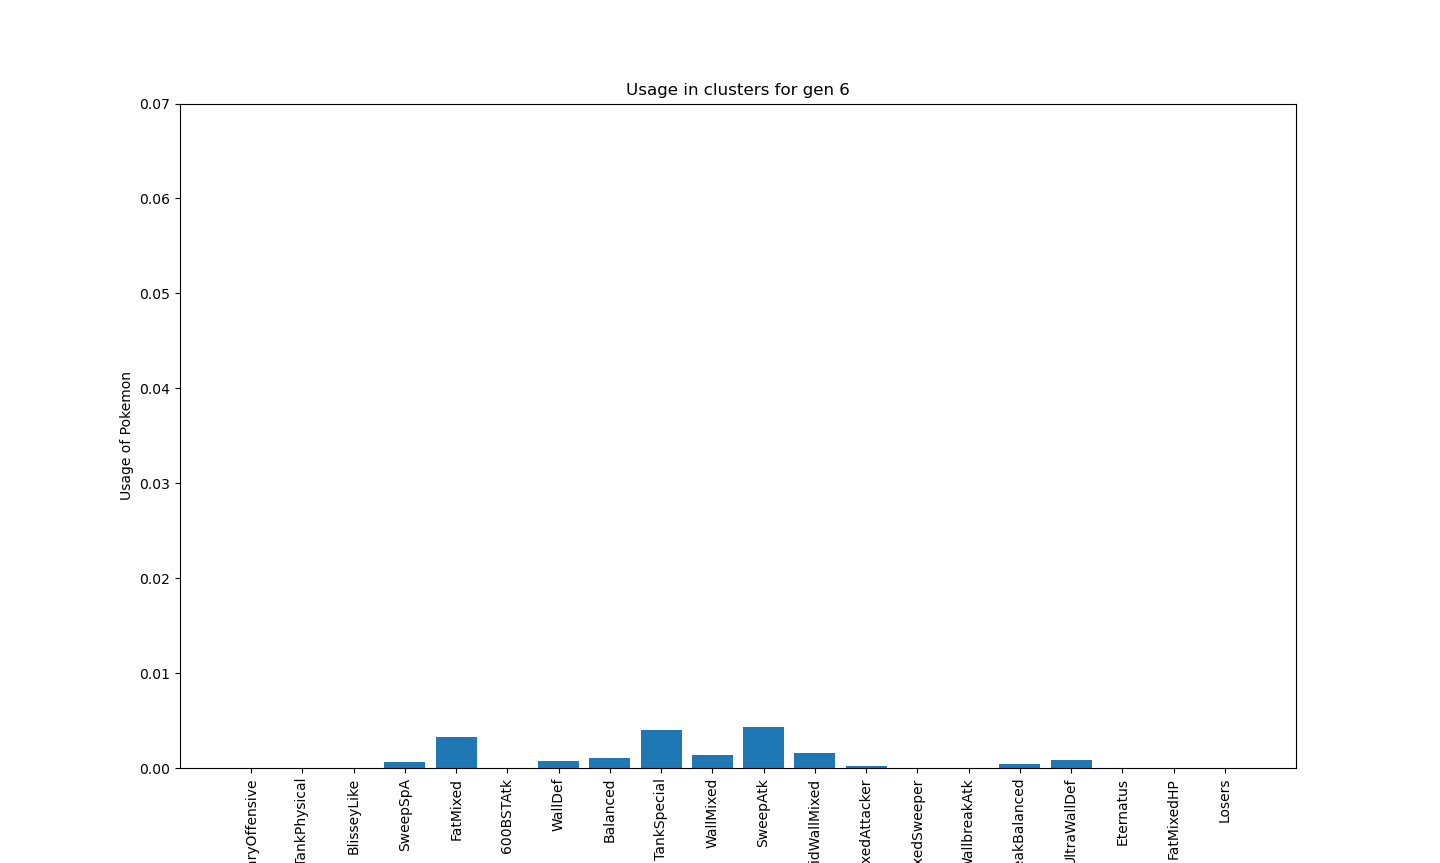
\includegraphics[width=0.45\textwidth]{Clustering/usage_gen/gen6.png}
    

    \vspace{1em}  % Ajoute un espace vertical entre les lignes

    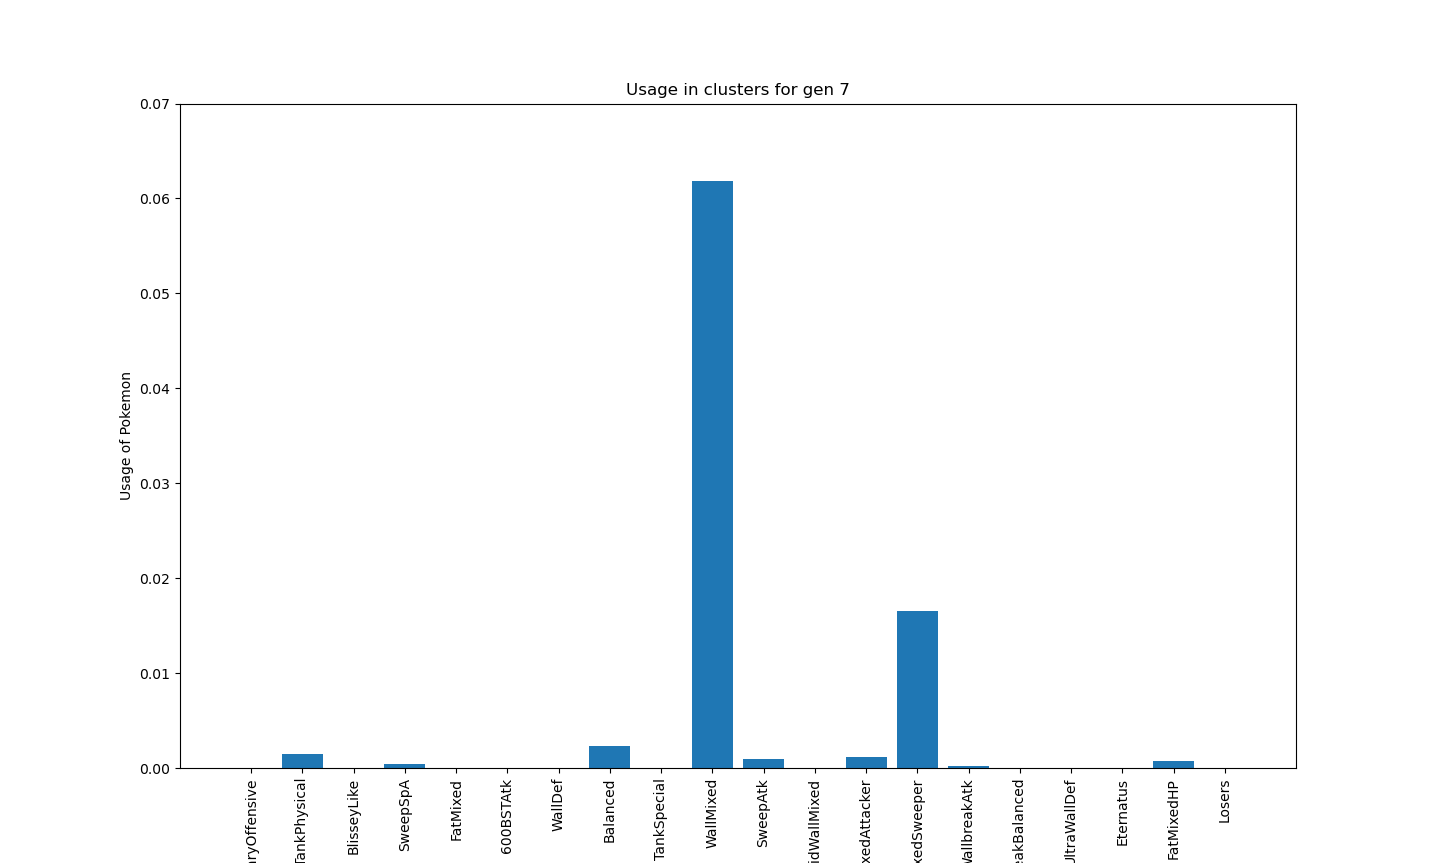
\includegraphics[width=0.45\textwidth]{Clustering/usage_gen/gen7.png}
    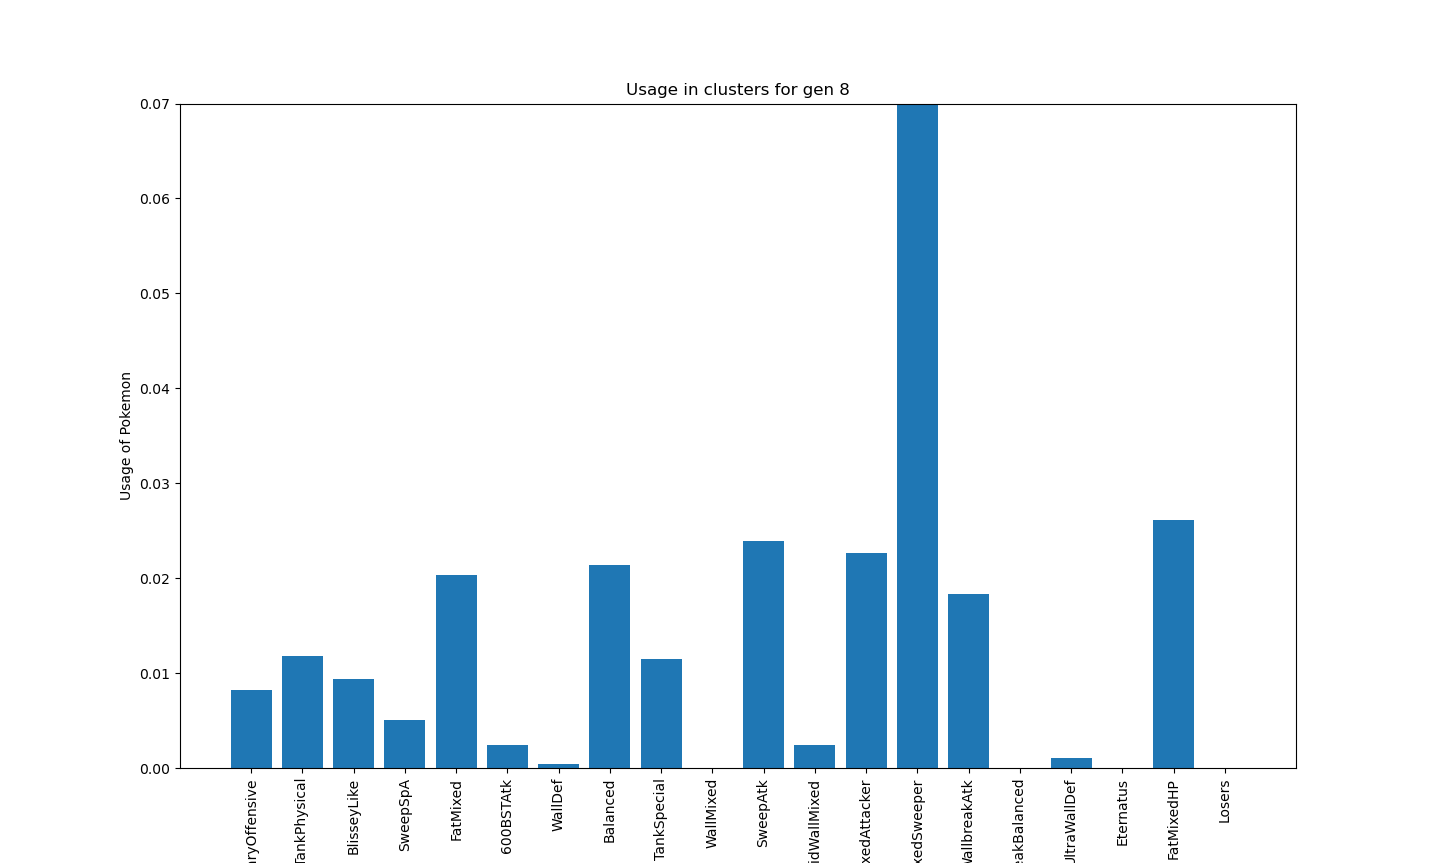
\includegraphics[width=0.45\textwidth]{Clustering/usage_gen/gen8.png}
    

    \vspace{1em}  % Ajoute un espace vertical entre les lignes

    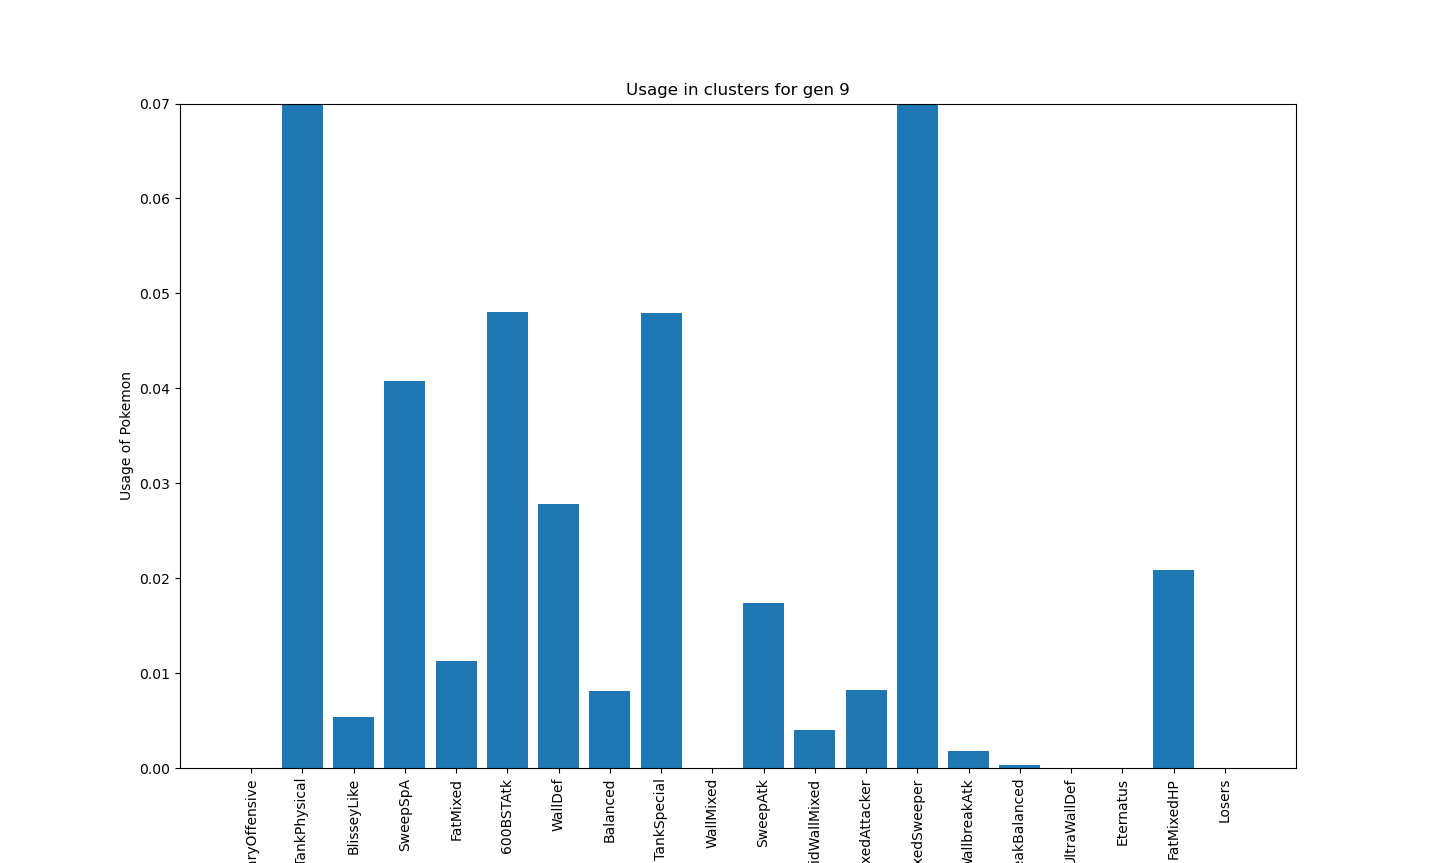
\includegraphics[width=0.45\textwidth]{Clustering/usage_gen/gen9.png}
    \caption*{Annexe 2 : Usage moyen d'un Pokémon au sein des clusters selon la génération}
\end{figure}


\end{document}
